\section{Multiple Life Models}
\label{sect:mult-life-models}
\begin{enumerate}
\item Multiple life model is a generalization by increasing the number of lives
involved in a single policy. So far, we have only considered the case with only
one life in a single policy, but in practice, a policy can involve more than
one lives, e.g., couple insurance (2 lives) and business partner insurance (2 or
more lives). How should we model such kind of products? The good
\faIcon[regular]{thumbs-up} news is that multiple life model can again be seen
as a special case of multiple state model, which allows us to recycle
results in \Cref{sect:mult-state-models}. So, like what we did in
\Cref{sect:mult-decr-models}, we will focus on concepts and formulas
specialized for the multiple life model here.

\item To illustrate how the multiple life model is a special case of multiple
state model, consider the case with 2 lives \emph{(main focus in
\Cref{sect:mult-life-models})}: \((x)\) (a life aged \(x\)) and \((y)\)
(another life aged \(y\)). In this case, the multiple life model can be
graphically represented as follows.
\begin{center}
\begin{tikzpicture}
\node[draw, minimum width=3cm, minimum height=1.5cm] () at (0,0) {Both alive (0)};
\node[draw, minimum width=3cm, minimum height=1.5cm] () at (7,0) {Only \((x)\) alive (1)};
\node[draw, minimum width=3cm, minimum height=1.5cm] () at (0,-3) {Only \((y)\) alive (2)};
\node[draw, minimum width=3cm, minimum height=1.5cm] () at (7,-3) {Both dead (3)};
\draw[-Latex] (1.5,0) --node[midway, above]{\((y)\) dies} (5.5,0);
\draw[-Latex] (7,-0.75) --node[midway, right]{\((x)\) dies} (7,-2.25);
\draw[-Latex] (0,-0.75) --node[midway, left]{\((x)\) dies} (0,-2.25);
\draw[-Latex] (1.5,-3) --node[midway, below]{\((y)\) dies} (5.5,-3);
\draw[-Latex] (1.5,-0.75) --node[midway]{die simultaneously} (5.5,-2.25);
\end{tikzpicture}
\end{center}
\begin{note}
By regarding ``\((x)\)'' and ``\((y)\)'' in the state names as labels for lives
\underline{originally} aged \(x\) and \(y\) respectively, the state names here
can still be used at later time (where the two lives are not aged \(x\) and
\(y\) respectively anymore).
\end{note}

\begin{warning}
There are different ways of labelling the states, so be careful about the
definition being used. Here we shall always adopt the labelling above for
multiple life model with 2 lives.
\end{warning}

For obvious reasons, all the directions here are one-directional. The
direct transition from state 0 to state 3 (simultaneous death) may occur when,
e.g., both lives die together in a car crash \faIcon{car-crash}.

Unless otherwise specified, throughout \Cref{sect:mult-life-models}, we will
work in \emph{continuous-time} multiple life models with \emph{2 lives}, where
transitions can take place at any time.
\end{enumerate}
\subsection{Probabilistic Calculations}
\label{subsect:mult-life-prob-calc}
\begin{enumerate}
\item\label{it:revised-mult-state-notations} \textbf{Revised multiple state
model notations.} Since there are more than one lives involved in a multiple
life model, we need to use a \emph{revised} version of the previous multiple
state model notations (like ``\(\px[t]{x}[ij]\)'', ``\(\mu_{x+t}^{ij}\)'',
``\(\Ax*{xy}[ij]\)'', etc.), so that the notations can carry the age information
from \underline{all} the lives involved.

To make the changes properly, the key \faIcon{key} is to look at the starting state:
\begin{itemize}
\item \emph{State 0:} Both lives are alive and involved, so we need to include
the ages for both of them in the post-subscript.
\item \emph{State 1:} Only the life originally aged \(x\) is alive and
involved, so we only need to include the age for that life in the post-subscript.
\item \emph{State 2:} Only the life originally aged \(y\) is alive and
involved, so we only need to include the age for that life in the post-subscript.
\end{itemize}
(We are not interested in studying quantities with starting state being 3.)

Examples:
\begin{itemize}
\item \(\px[t]{x}[0j]\to\px[t]{\rc{xy}}[0j],\quad\mu_{x}^{0j}\to\mu_{\rc{xy}}^{0j}\).

\begin{note}
When we replace \(x\) and \(y\) by actual numbers, we should add a colon to
separate them. For example, we should write \(\px[t]{\rc{20:30}}[0j]\) rather
than ``\(\px[t]{\rc{2030}}[0j]\)'' \(\leftarrow\) a life aged \(2030\)???
\end{note}
\item \(\px[s]{x+t}[0j]\to\px[s]{\rc{x+t:y+t}}[0j],\quad\mu_{x+t}^{0j}\to\mu_{\rc{x+t:y+t}}^{0j}\).
\item \(\px[t]{x}[2j]\to\px[t]{\rc{y}}[2j],\quad\mu_{x}^{2j}\to\mu_{\rc{y}}^{2j}\).
\item \(\px[s]{x+t}[2j]\to\px[s]{\rc{y+t}}[2j],\quad\mu_{x+t}^{2j}\to\mu_{\rc{y+t}}^{2j}\).

\item \(\px[t]{x}[\overline{00}]\to\px[t]{\rc{xy}}[\overline{00}],\quad
\px[t]{x}[0\bullet]\to\px[t]{\rc{xy}}[0\bullet],\quad
\mu_{x+t}^{0\bullet}\to\mu_{\rc{x+t:y+t}}^{0\bullet}\).

\begin{note}
Here, ``\(0\bullet\)'' quantity refers to the sum of all corresponding ``\(0j\)''
quantities with \(j=1,2,3\).
\end{note}
\item \(\Ax*{\endowxn}[03]\to\Ax*{\rc{xy}:\angl{n}}[03],\quad \ax**{x}[00]\to\ax**{\rc{xy}}[00]\).
\end{itemize}

\item \textbf{Specialized occupancy probability formulas.} Recall the occupancy
probability formula from \labelcref{it:occup-fmla}:
\[
\px[t]{x}[\overline{ii}]=\exp\qty(-\int_{0}^{t}\sum_{j\rc{\ne i}}^{}\mu_{x+s}^{ij}\dd{s}).
\]
In the multiple life model setting, we can simplify it to get:
\begin{itemize}
\item \(\displaystyle \px[t]{xy}[00]=\px[t]{xy}[\overline{00}]=\exp\qty(-\int_{0}^{t}\mu_{x+s:y+s}^{0\bullet}\dd{s})\).
\item \(\displaystyle \px[t]{x}[11]=\px[t]{x}[\overline{11}]=\exp\qty(-\int_{0}^{t}\mu_{x+s}^{13}\dd{s})\).
\item \(\displaystyle \px[t]{y}[22]=\px[t]{y}[\overline{22}]=\exp\qty(-\int_{0}^{t}\mu_{y+s}^{23}\dd{s})\).
\end{itemize}
\item \textbf{Specialized transition probability formulas.} Simplifying the
general transition probability formula from \labelcref{it:gen-tran-prob-fmla}:
\[
\px[t]{x}[ij]=\int_{0}^{t}\qty(\sum_{k\ne j}^{}\px[s]{x}[ik]\mu_{x+s}^{kj})
\px[t-s]{x+s}[\overline{jj}]\dd{s},
\]
we get:
\begin{itemize}
\item \(\displaystyle \px[t]{xy}[01]=\int_{0}^{t}\px[s]{x}[00]\times \mu_{x+s:y+s}^{01}\times \px[t-s]{x+s}[11]\dd{s}\).
\item \(\displaystyle \px[t]{xy}[02]=\int_{0}^{t}\px[s]{x}[00]\times \mu_{x+s:y+s}^{02}\times \px[t-s]{x+s}[22]\dd{s}\).
\item \(\displaystyle \px[t]{xy}[03]=\int_{0}^{t}\qty(\px[s]{xy}[00]\mu_{x+s:y+s}^{03}
+\px[s]{xy}[01]\mu_{x+s}^{13}
+\px[s]{xy}[02]\mu_{y+s}^{23}
)\dd{s}\).
\item \(\displaystyle \px[t]{x}[13]=\int_{0}^{t}\px[s]{x}[11]\mu_{x+s}^{13}\dd{s}\).
\item \(\displaystyle \px[t]{y}[23]=\int_{0}^{t}\px[s]{y}[22]\mu_{y+s}^{23}\dd{s}\).
\end{itemize}
\begin{remark}
\item It is impossible to leave state \(3\) once it is entered.
\item Be careful about the post-subscripts of the notations.
\end{remark}
\item \textbf{Random variable approach to multiple life model.} Like multiple
decrement model, multiple life model can be handled using a random variable
approach. The idea is to (as expected) introduce multiple future lifetime
random variables, one for each life.

Let \(T_x\) and \(T_y\) denote the (\underline{not} necessarily independent
\warn{}) future lifetime random variables of \((x)\) and \((y)\) respectively.
When considering \(T_x\) and \(T_y\) \emph{individually} (marginal
distributions), we are back to the case in STAT3901 where the notations there
would apply (e.g., \(\px[t]{x}=\prob{T_x>t}, \qx[t]{y}=\prob{T_y\le t}\),
etc.). But here, in multiple life model, we are more interested in their
\emph{joint} behaviour and \emph{joint} distribution. Particularly, we are
going to study two ways of ``combining'' the two lifetimes together: (i)
joint-life status and (ii) last-survivor status.

\item \textbf{Joint-life status.} The idea of \emph{joint-life status} is to
``join'' or ``link'' \faIcon{link} the two lives together. The \rc{death}
\faIcon{skull} of one of the lives would ``break the link'' \faIcon{unlink},
and in such case the joint-life status is deemed to ``fail''.

The \defn{joint-life status} of two lives \((x)\) and \((y)\), denoted by
\((xy)\) (or \((x\!:\!y)\) if it looks better), is said to \emph{fail} when
\underline{one of the lives} \rc{dies} \faIcon{skull}. Let \(T_{xy}\) denote
the time to failure of the joint-life status \((xy)\). By treating ``fail''
as ``die'' and ``not fail'' as ``survive'', we may regard \((xy)\) as a
``special life'' and \(T_{xy}\) as its ``future lifetime''. By definition, we
have \(T_{xy}=T_x\wedge T_y=\min\{T_x,T_y\}\).

Using the concept of joint-life status, we can (finally!) explain the rationale
behind the seemingly strange ``\(\endowxn\)'' notations appearing in STAT3901
(e.g., endowment insurance EPV \(\Ax*{\vc{\endowxn}}\) and temporary life
annuity EPV \(\ax*{\vc{\endowxn}}\)).  The underlying idea is to treat
``\((\angl{n})\)'' as a ``life'' whose ``lifetime'' is \emph{certainly} \(n\)
years, i.e., ``\(T_{\angl{n}}=n\)'' always. Hence, the ``future lifetime'' of
the ``joint-life status'' \((\endowxn)\) is \(T_{\endowxn}=T_x\wedge
T_{\angl{n}}=T_x\wedge n\).  Then, for example, we can treat an \(n\)-year
endowment insurance issued to \((x)\) as a whole life insurance issued to
``\((\endowxn)\)'', which explains the notation ``\(\Ax*{\endowxn}\)''.

\item \textbf{Last-survivor status.} The idea of \emph{last-survivor status} is
to, as its name suggests, represent the status of last survivor. When the last
survivor \rc{dies} \faIcon{skull}, the status is deemed to ``fail''.

The \defn{last-survivor status} of two lives \((x)\) and \((y)\), denoted by
\((\overline{xy})\) (or \((\overline{x\!:\!y})\) if it looks better), is said
to \emph{fail} when \underline{all lives} \rc{die} \faIcon{skull}\faIcon{skull}
(equivalently, the last survivor dies). Let \(T_{\overline{xy}}\) denote the
time to failure of the last-survivor status. Like joint-life status,
\((\overline{xy})\) can be treated as a ``special life'' with ``future
lifetime'' being \(T_{\overline{xy}}\), when we regard ``fail'' as ``die'' and
``not fail'' as ``survive''. By definition, we have \(T_{\overline{xy}}=T_x\vee
T_y=\max\{T_x,T_y\}\).

\item \textbf{Joint-life and last-survivor statuses for more than two lives.}
Joint-life and last-survivor statuses can be naturally extended to the case
with more than two lives. Suppose there are \(m\) lives \((x_1),\dotsc,(x_m)\).
Their joint-life status is denoted by \((x_1\cdots x_m)\) and we have
\(T_{x_1\cdots x_m}=\min\{T_{x_1},\dotsc,T_{x_m}\}\); Their last-survivor
status is denoted by \((\overline{x_1\cdots x_m})\) and we have
\(T_{\overline{x_1\cdots x_m}}=\max\{T_{x_1},\dotsc,T_{x_m}\}\).

Although this works for any number of lives, very often the maximum number of
lives we are asked to deal with is 3.

\item \textbf{Combining multiple joint-life and last-survivor statuses.}
Since joint-life and last-survivor statuses can be treated as ``special
lives'', it is possible to combine multiple statuses by considering
joint-life/last-survivor status of two ``special lives''. For example:
\begin{itemize}
\item Joint-life status of two ``special lives'' \((xy)\) and \((wz)\):
\begin{itemize}
\item \emph{Notation:} \((xy\!:\!wz)\) (or \((x\!:\!y\!:\!w\!:\!z)\)).
\item \emph{Time to failure:} \(T_{xy:wz}=\min\{T_{xy},T_{wz}\}=\min\{T_{x},T_{y},T_{w},T_{z}\}\).
\end{itemize}
Note that we can ``simplify'' this bulky joint-life status to a ``simpler''
joint-life status of 4 lives: \((x)\), \((y)\), \((w)\), and \((z)\).
\item Last-survivor status of two ``special lives'' \((\overline{xy})\) and \((\overline{wz})\):
\begin{itemize}
\item \emph{Notation:} \((\overline{\overline{xy}\!:\!\overline{wz}})\)
(or \((\overline{\overline{x\!:\!y}\!:\!\overline{w\!:\!z}})\)).
\item \emph{Time to failure}
\(T_{\overline{xy:wz}}=\max\{T_{\overline{xy}},T_{\overline{wz}}\}
=\max\{T_{x},T_{y},T_{w},T_{z}\}\).
\end{itemize}
Note that we can ``simplify'' this bulky last-survivor status to a ``simpler''
last-survivor status of 4 lives: \((x)\), \((y)\), \((w)\), and \((z)\).

\item Last-survivor status of two ``special lives'' \((\overline{xy})\) and \((wz)\):
\begin{itemize}
\item \emph{Notation:} \((\overline{\overline{xy}\!:\!wz})\)
\item \emph{Time to failure:}
\(T_{\overline{\overline{xy}:wz}}=\max\{T_{\overline{xy}},T_{wz}\}
=\max\{\max\{T_x,T_y\},\min\{T_w,T_z\}\}\).
\end{itemize}

\end{itemize}
Things would get complicated quickly as we combine more statuses together, so
let us stop here.

\subsubsection*{Revisiting Survival Model Topics for Joint-Life and Last-Survivor Statuses}
\item As we associate joint-life and last-survivor statuses with ``special
lives'', and associate time to failure with ``future lifetime'', we can study
numerous aspects about the joint-life and last-survivor statuses by revisiting
the following topics about survival models from STAT3901 (with slight changes
in names):
\begin{itemize}
\item probabilities about \sout{future lifetime} time to failure
\item force of \sout{mortality} failure
\item curtate \sout{future lifetime} time to failure
\item moments of \sout{future lifetimes} time to failure
\item recursions for expectations of \sout{life} time to failure
\end{itemize}
\begin{note}
We will focus on the case with 2 lives for simplicity, but similar developments
can be done for the cases with more lives.
\end{note}

\item\label{it:fail-time-prob} \textbf{Probabilities about time to failure.}
\begin{enumerate}[label={(\arabic*)}]
\item \emph{Notations:} The probability notations from STAT3901 can be recycled
for the joint-life and last-survivor statuses, by treating them as ``special
lives'':
\begin{center}
\begin{tabular}{ll}
\toprule
Notation&Probability that ...\\
\midrule
\(\px[t]{xy}=S_{xy}(t)=\prob{T_{xy}>t}\)&\((xy)\) \gc{``survives''} \(t\) years \\
\(\qx[t]{xy}=F_{xy}(t)=\prob{T_{xy}\le t}\)&\((xy)\) \rc{``dies''} within \(t\) years\\
\(\qx[u|t]{xy}=\prob{u<T_{xy}\le u+t}\)&\((xy)\) \gc{``survives''} \(u\) years 
and \rc{``dies''} in the subsequent \(t\) years\\
\(\px[t]{\overline{xy}}=S_{\overline{xy}}(t)=\prob{T_{\overline{xy}}>t}\)
&\((\overline{xy})\) \gc{``survives''} \(t\) years \\
\(\qx[t]{\overline{xy}}=F_{\overline{xy}}(t)=\prob{T_{\overline{xy}}\le t}\)
&\((\overline{xy})\) \rc{``dies''} within \(t\) years\\
\(\qx[u|t]{\overline{xy}}=\prob{u<T_{\overline{xy}}\le u+t}\)
&\((\overline{xy})\) \gc{``survives''} \(u\) years 
and \rc{``dies''} in the subsequent \(t\) years\\
\bottomrule
\end{tabular}
\end{center}
\item \emph{Key formulas:}
\begin{enumerate}[label={(\roman*)}]
\item \emph{Factorization formula for ``\(p\)'' for \textbf{joint-life status}:}
\[\underbrace{\px[t+u]{xy}}_{\text{``survive'' \(t+u\) yrs.}}
=\underbrace{\px[t]{xy}}_{\text{``survive'' \(t\) yrs.\ first}}\times 
\underbrace{\px[u]{x+t:y+t}}_{\text{then ``survive'' \(u\) more yrs.}}.
\footnote{\emph{(If you are interested)} Like the case for STAT3901, this can
be proven mathematically by considering conditional probability, with the
natural assumption that \(T_{xy}-t|T_{xy}>t\eqd T_{x+t:y+t}\), where
``\(\eqd\)'' denotes equality in distribution. Note that it does NOT make sense
to impose an analogous definition for last-survivor status \warn{}, due to the
reason discussed in the ``warning'' part.}\]
\begin{warning}
We do NOT have a corresponding formula for last-survivor status like below:
\[\px[t+u]{\overline{xy}}
=\px[t]{\overline{xy}}\times 
\px[u]{\overline{x+t:y+t}}.\]
The key issue is that, after \((\overline{xy})\) ``survives'' \(t\) years, it
may NOT become \((\overline{x+t\!:\!y+t})\) \warn{}. This is because
``surviving'' \(t\) years here just means the last-survivor status
\((\overline{xy})\) does \emph{not} fail for \(t\) years, i.e., \emph{not all}
lives die within \(t\) years. It is possible for \emph{exactly one} life to die
\faIcon{skull} within \(t\) years! In such situation,
``\((\overline{x+t\!:\!y+t})\)'' does not make sense anymore as it is defined
on the condition that both lives are alive (NOT the case here!).

On the other hand, the joint-life status does not have such issue, since after
\((xy)\) ``survives'' \(t\) years, it indeed becomes
\((x+t\!:\!y+t)\), like a ``normal'' life. This is because not
failing for \(t\) years really means both lives survive \(t\) years in the
joint-life status case.
\end{warning}
\item \emph{Formulas for ``\(\qx[u|t]{\square}\)'':}

\textbf{Joint-life status:}
\begin{itemize}
\item \emph{``\(\gc{p}\times \rc{q}\)'' form:} 
\[\qx[u|t]{xy}=\underbrace{\gc{\px[u]{xy}}}_{\text{``survive'' \(u\) yrs.}}
\times \underbrace{\rc{\qx[t]{x+u:y+u}}}_{\text{``die'' in the subsequent \(t\) yrs.}}\]
\item \emph{``\(\gc{p}-\gc{p}\)'' form:}
\[
\qx[u|t]{xy}=\underbrace{\gc{\px[u]{xy}}}_{\text{``survive'' \(u\) yrs.}}
\;\underbrace{-\gc{\px[u+t]{xy}}}_{\text{but not ``survive'' \(u+t\) yrs}}
\]
\item \emph{``\(\rc{q}-\rc{q}\)'' form:}
\[
\qx[u|t]{xy}=\underbrace{\rc{\qx[u+t]{xy}}}_{\text{``die'' in \(u+t\) yrs.}}\;
\underbrace{-\rc{\qx[u]{xy}}}_{\text{but not ``die'' in \(u\) yrs.}}
\]
\end{itemize}

\textbf{Last-survivor status:}
\begin{itemize}
\item \emph{``\(\gc{p}-\gc{p}\)'' form:}
\[
\qx[u|t]{\overline{xy}}=\underbrace{\gc{\px[u]{\overline{xy}}}}_{\text{``survive'' \(u\) yrs.}}
\;\underbrace{-\gc{\px[u+t]{\overline{xy}}}}_{\text{but not ``survive'' \(u+t\) yrs}}
\]
\item \emph{``\(\rc{q}-\rc{q}\)'' form:}
\[
\qx[u|t]{\overline{xy}}=\underbrace{\rc{\qx[u+t]{\overline{xy}}}}_{\text{``die'' in \(u+t\) yrs.}}\;
\underbrace{-\rc{\qx[u]{\overline{xy}}}}_{\text{but not ``die'' in \(u\) yrs.}}
\]
\end{itemize}
\begin{warning}
Due to the same reason as above, we do NOT have ``\(\gc{p}\times \rc{q}\)''
form for last-survivor status.
\end{warning}
\item \emph{(new!) \(\text{Joint-life}+\text{Last-survivor}=\text{Individual sum}\):}
\begin{itemize}
\item \(\px[t]{xy}+\px[t]{\overline{xy}}=\px[t]{x}+\px[t]{y}\).
\item \(\qx[t]{xy}+\qx[t]{\overline{xy}}=\qx[t]{x}+\qx[t]{y}\).
\item \emph{(density functions)} \(f_{xy}(t)+f_{\overline{xy}}(t)=f_{x}(t)+f_{y}(t)\).
\end{itemize}
\begin{note}
These follow from the inclusion-exclusion principle of probability.
\end{note}
\item \emph{(new!) Inclusion-exclusion type formulas:} Here we consider the
case with 3 lives \((x)\), \((y)\), and \((z)\). Denote
\(\px[t]{xyz}=\prob{T_{xyz}>t}\), \(\qx[t]{xyz}=\prob{T_{xyz}\le t}\),
\(\px[t]{\overline{xyz}}=\prob{T_{\overline{xyz}}>t}\), and
\(\qx[t]{\overline{xyz}}=\prob{T_{\overline{xyz}}\le t}\). Then we have:
\begin{itemize}
\item \(\qx[t]{xyz}=\qx[t]{x}+\qx[t]{y}+\qx[t]{z}-\qx[t]{\overline{xy}}-\qx[t]{\overline{xz}}
-\qx[t]{\overline{yz}}+\qx[t]{\overline{xyz}}\).

\item \(\px[t]{xyz}=\px[t]{x}+\px[t]{y}+\px[t]{z}-\px[t]{\overline{xy}}-\px[t]{\overline{xz}}
-\px[t]{\overline{yz}}+\px[t]{\overline{xyz}}\).

\item \(\qx[t]{\overline{xyz}}=\qx[t]{x}+\qx[t]{y}+\qx[t]{z}-\qx[t]{xy}-\qx[t]{xz}
-\qx[t]{yz}+\qx[t]{xyz}\).

\item \(\px[t]{\overline{xyz}}=\px[t]{x}+\px[t]{y}+\px[t]{z}-\px[t]{xy}-\px[t]{xz}
-\px[t]{yz}+\px[t]{xyz}\).
\end{itemize}
\begin{note}
Not surprisingly, these again follow from the inclusion-exclusion principle of
probability.
\end{note}
\end{enumerate}
\end{enumerate}
\item \textbf{Force of failure.}
\begin{enumerate}[label={(\arabic*)}]
\item \emph{Definitions:} The \defn{force of failure} \faIcon{at} time \(t\) is
defined by:
\begin{itemize}
\item \emph{Joint-life status:}
\(\displaystyle \mu_{xy}(t)=-\frac{S_{xy}'(t)}{S_{xy}(t)}=-\frac{\dv{}{t}\px[t]{xy}}{\px[t]{xy}}\).
\item \emph{Last-survivor status:}
\(\displaystyle \mu_{\overline{xy}}(t)=-\frac{S_{\overline{xy}}'(t)}{S_{\overline{xy}}(t)}
=-\frac{\dv{}{t}\px[t]{\overline{xy}}}{\px[t]{\overline{xy}}}\).
\end{itemize}

\item \emph{Interpretations:} The forces of failure here share similar
interpretations to the force of mortality:
\begin{itemize}
\item \(\mu_{xy}(t)\Delta t\): approximated probability for \((xy)\) to
\rc{fail} in the time interval \([t,t+\Delta t]\), when \(\Delta t\) is small.
\item \(\mu_{\overline{xy}}(t)\Delta t\): approximated probability for
\((\overline{xy})\) to \rc{fail} in the time interval \([t,t+\Delta t]\), when
\(\Delta t\) is small.
\end{itemize}
\item \emph{Key formulas:}
\begin{enumerate}[label={(\roman*)}]
\item \emph{\(\text{Force of failure \(\mu_{\square}\)}\to\text{survival function \(\px[t]{\square}\)}\):}
\begin{itemize}
\item \emph{(joint-life status)}
\[
\px[t]{xy}=\exp\qty(-\int_{0}^{t}\mu_{xy}(s)\dd{s}).\]

\item \emph{(last-survivor status)}
\[
\px[t]{\overline{xy}}=\exp\qty(-\int_{0}^{t}\mu_{\overline{xy}}(s)\dd{s}).
\]
\end{itemize}
\item \emph{Density functions:}
\begin{itemize}
\item \emph{(joint-life status)} \(f_{xy}(t)=\px[t]{xy}\times \mu_{xy}(t)\).
\item \emph{(last-survivor status)} \(f_{\overline{xy}}(t)=\px[t]{\overline{xy}}\times \mu_{\overline{xy}}(t)\).
\end{itemize}
\end{enumerate}
\end{enumerate}
\item \textbf{Curtate time to failure.}
\begin{enumerate}[label={(\arabic*)}]
\item \emph{Definitions:} The \defn{curtate time to failure} is defined by:
\begin{itemize}
\item \emph{Joint-life status:} \(K_{xy}=\lfloor T_{xy}\rfloor\).
\item \emph{Last-survivor status:} \(K_{\overline{xy}}=\lfloor T_{\overline{xy}}\rfloor\).
\end{itemize}
\item \emph{Key formulas:}
\begin{enumerate}[label={(\roman*)}]
\item \emph{Mass functions:}
\begin{itemize}
\item \emph{(joint-life status)} \(\displaystyle \prob{K_{xy}=k}=\qx[k|]{xy}=\begin{cases}
\text{``\(\gc{p}\times \rc{q}\)'' form ...} \\
\text{``\(\gc{p}-\gc{p}\)'' form ...} \\
\text{``\(\rc{q}-\rc{q}\)'' form ...}
\end{cases}
\).
\item \emph{(last-survivor status)} \(\displaystyle \prob{K_{\overline{xy}}=k}=\qx[k|]{\overline{xy}}
=\begin{cases}
\text{\sout{``\(\gc{p}\times \rc{q}\)'' form ...}} \\
\text{``\(\gc{p}-\gc{p}\)'' form ...} \\
\text{``\(\rc{q}-\rc{q}\)'' form ...}
\end{cases}
\).
\end{itemize}
\item \emph{Cumulative distribution functions:}
\begin{itemize}
\item \emph{(joint-life status)} \(\prob{K_{xy}\le k}=\qx[\rc{k+1}]{xy}\).
\item \emph{(last-survivor status)} \(\prob{K_{\overline{xy}}\le k}=\qx[\rc{k+1}]{\overline{xy}}\).
\end{itemize}
\end{enumerate}
\end{enumerate}
\item \label{it:fail-time-moments} \textbf{Moments of time to failure.}
\begin{enumerate}[label={(\arabic*)}]
\item \emph{Notations:}
\begin{center}
\begin{tabular}{ll}
\toprule
Notation&Meaning \\
\midrule
\(\eringx{xy}\)&\(\expv{T_{xy}}\) \\
\(\eringx{\overline{xy}}\)&\(\expv{T_{\overline{xy}}}\) \\
\(e_{xy}\)&\(\expv{K_{xy}}\) \\
\(e_{\overline{xy}}\)&\(\expv{K_{\overline{xy}}}\) \\
\bottomrule
\end{tabular}
\begin{tabular}{ll}
\toprule
Notation&Meaning \\
\midrule
\(\eringx{xy:\angl{n}}\)&\(\expv{T_{xy}\wedge n}\) \\
\(\eringx{\overline{xy}:\angl{n}}\)&\(\expv{T_{\overline{xy}}\wedge n}\) \\
\(e_{xy:\angl{n}}\)&\(\expv{K_{xy}\wedge n}\) \\
\(e_{\overline{xy}:\angl{n}}\)&\(\expv{K_{\overline{xy}}\wedge n}\) \\
\bottomrule
\end{tabular}
\end{center}
\item \emph{Key formulas:} \((\square = xy\text{ or }\overline{xy})\)
\begin{enumerate}[label={(\roman*)}]
\item \emph{Shortcut formulas for expectation:}
\begin{itemize}
\item \(\displaystyle \eringx{\square}=\int_{0}^{\infty}\px[t]{\square}\dd{t}\).
\item \(\displaystyle e_{\square}=\sum_{k=\rc{1}}^{\infty}\px[k]{\square}\).
\end{itemize}
\item \emph{Shortcut formulas for temporary expectation:}
\begin{itemize}
\item \(\displaystyle \eringx{\square:\angl{n}}=\int_{0}^{n}\px[t]{\square}\dd{t}\).
\item \(\displaystyle e_{\square:\angl{n}}=\sum_{k=\rc{1}}^{n}\px[k]{\square}\).
\end{itemize}
\item \emph{(Less commonly used) Shortcut formulas for second moment:}
\begin{itemize}
\item \(\displaystyle \expv{T_{\square}^{2}}=\int_{0}^{\infty}2t\times \px[t]{\square}\dd{t}\).
\item \(\displaystyle \expv{K_{\square}^{2}}=\sum_{k=\rc{1}}^{\infty}(2k-1)\px[k]{\square}\).
\end{itemize}
\item \emph{(new!) \(\text{Joint-life}+\text{Last-survivor}=\text{Individual sum}\):}
\begin{itemize}
\item \(\eringx{xy}+\eringx{\overline{xy}}=\eringx{x}+\eringx{y}\).
\item \(e_{xy}+e_{\overline{xy}}=e_{x}+e_{y}\).
\end{itemize}
\begin{note}
These follow from the identity \(T_{xy}+T_{\overline{xy}}\equiv T_x+T_y\).
\end{note}
\item \emph{(new!) Covariance formula:}
\[
\cov{T_{xy}}{T_{\overline{xy}}}=\cov{T_x}{T_y}+(\eringx{x}-\eringx{xy})(\eringx{y}-\eringx{xy})
\]
\begin{pf}
(Sketch) The key is to first note the identity \(T_{xy}T_{\overline{xy}}\equiv
T_xT_y\), and then write
\[
\cov{T_{xy}}{T_{\overline{xy}}}=
\underbrace{\expv{\vc{T_xT_y}}\blc{-\expv{T_x}\expv{T_y}}}_{\cov{T_x}{T_y}}
\underbrace{\blc{+\expv{T_x}\expv{T_y}}
-\expv{T_{xy}}\expv{\vc{T_{x}+T_{y}-T_{xy}}}}_{(\eringx{x}-\eringx{xy})(\eringx{y}-\eringx{xy})
}.
\]
\end{pf}
\end{enumerate}
\end{enumerate}
\item \textbf{Recursions for expectations of time to failure.} In general,
recursions only work for \emph{joint-life status}, but NOT for last-survivor
status \warn{}, due to the reason discussed before in
\labelcref{it:fail-time-prob}.

\emph{Recursive formulas:}
\begin{itemize}
\item \(\eringx{xy}=\eringx{xy:\angl{n}}+\px[n]{xy}\eringx{x+n:y+n}\)
\item \(e_{xy}=e_{xy:\angl{n}}+\px[n]{xy}e_{x+n:y+n}\overset{(n=1)}{=}p_{xy}(1+e_{x+1:y+1})\)
\item \(\eringx{xy:\angl{n}}\overset{(m\le n)}{=}\eringx{xy:\angl{m}}+\px[m]{xy}\eringx{x+m:y+m:\angl{n-m}}\)
\item \(e_{xy:\angl{n}}\overset{(m\le n)}{=}e_{x:\angl{m}}+\px[m]{xy}e_{x+m:y+m:\angl{n-m}}
\overset{(m=1)}{=}p_{xy}(1+e_{x+1:y+1:\angl{n-1}})\)
\end{itemize}
\begin{note}
\(\eringx{x+m:y+m:\angl{n-m}}\) can be treated as \(\expv{T_{x+m:y+m}\wedge
(n-m)}\) or \(\expv{T_{x+m:y+m:\angl{n-m}}}\) without ambiguity, as both of
them actually mean the same.
\end{note}
\subsubsection*{Translating between multiple state and random variable approach notations}
\item After revisiting the survival model topics, we have accumulated enough
``ingredients'' to discuss how we can ``translate'' between the multiple state
notations and the notations based on random variable approach.

\item \textbf{Translation between probability notations.}
A handy visual tool that helps us to do the translation in this case is the
following picture:
\begin{center}
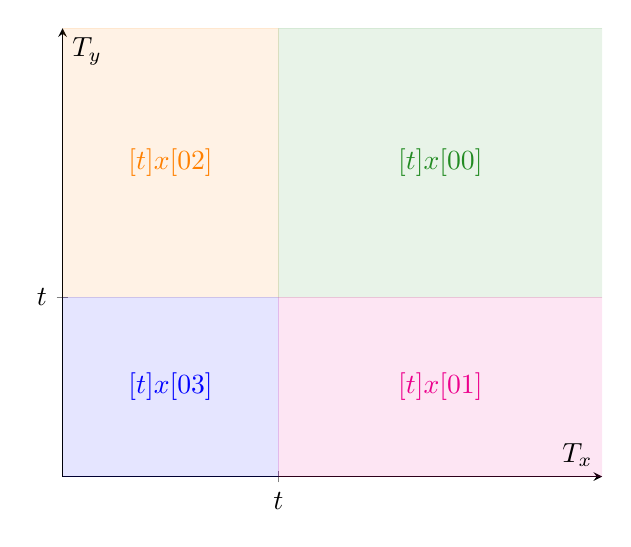
\begin{tikzpicture}
\begin{axis}[xmin=0, ymin=0, xmax=5, ymax=5,
xtick={2}, ytick={2}, xticklabels={\(t\)}, yticklabels={\(t\)}, axis lines=middle,
xlabel={\(T_x\)}, ylabel={\(T_y\)}]
\draw[fill, ForestGreen, opacity=0.1] (2,2) rectangle (5,5);
\draw[fill, magenta, opacity=0.1] (2,2) rectangle (5,0);
\draw[fill, orange, opacity=0.1] (0,2) rectangle (2,5);
\draw[fill, blue, opacity=0.1] (0,0) rectangle (2,2);
\node[blue] () at (1,1) {\(\px[t]{x}[03]\)};
\node[orange] () at (1,3.5) {\(\px[t]{x}[02]\)};
\node[magenta] () at (3.5,1) {\(\px[t]{x}[01]\)};
\node[ForestGreen] () at (3.5,3.5) {\(\px[t]{x}[00]\)};
\end{axis}
\end{tikzpicture}
\end{center}
This suggests the correspondence between multiple state transition
probabilities and the events for the random variable approach. Using this
picture, we can deduce, for example:
\begin{itemize}
\item \(\px[t]{x}=\prob{T_x>t}=\gc{\px[t]{x}[00]}+\mgc{\px[t]{x}[01]}\).
\item \(\px[t]{y}=\prob{T_y>t}=\gc{\px[t]{x}[00]}+\orc{\px[t]{x}[02]}\).
\item \(\px[t]{xy}=\prob{T_x>t\cap T_y>t}=\gc{\px[t]{x}[00]}\).
\item \(\qx[t]{\overline{xy}}=\prob{T_x\le t\cap T_y\le t}=\blc{\px[t]{x}[03]}\).
\end{itemize}
\begin{center}
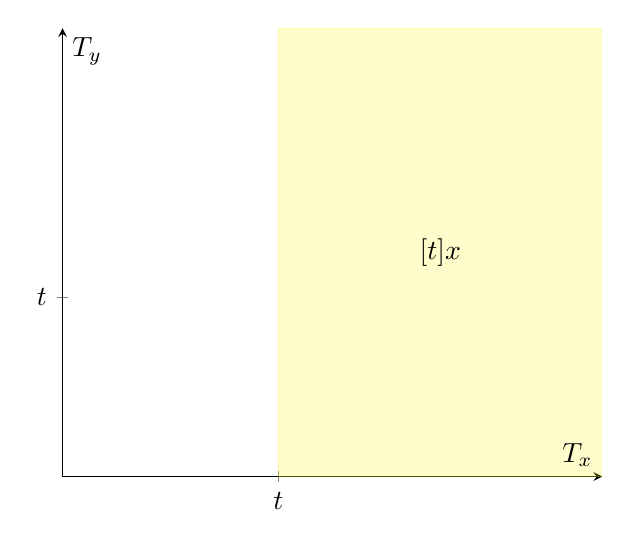
\begin{tikzpicture}[]
\begin{axis}[xmin=0, ymin=0, xmax=5, ymax=5,
xtick={2}, ytick={2}, xticklabels={\(t\)}, yticklabels={\(t\)}, axis lines=middle,
xlabel={\(T_x\)}, ylabel={\(T_y\)}]
\draw[fill, yellow, opacity=0.2] (2,0) rectangle (5,5);
\node[] () at (3.5,2.5) {\(\px[t]{x}\)};
\end{axis}
\end{tikzpicture}
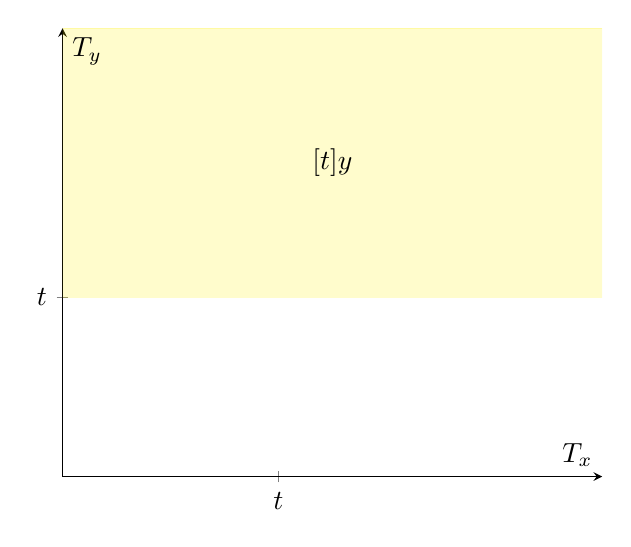
\begin{tikzpicture}[]
\begin{axis}[xmin=0, ymin=0, xmax=5, ymax=5,
xtick={2}, ytick={2}, xticklabels={\(t\)}, yticklabels={\(t\)}, axis lines=middle,
xlabel={\(T_x\)}, ylabel={\(T_y\)}]
\draw[fill, yellow, opacity=0.2] (0,2) rectangle (5,5);
\node[] () at (2.5,3.5) {\(\px[t]{y}\)};
\end{axis}
\end{tikzpicture}
\end{center}
\item \textbf{Translation between forces of transition/failure.}
In multiple life model, there are two types of ``forces'': (i) force of
transition (for multiple state approach) and (ii) force of failure (for random
variable approach). One would naturally expect them to have some relationships,
and that is indeed the case. First we introduce some extra notations:
\[\mu_{x+t:y+t}:=\mu_{x+t:y+t}(0),\quad
\mu_{\overline{x+t:y+t}}:=\mu_{\overline{x+t:y+t}}(0).\footnote{
\emph{(If you are interested)} To better understand the rationale behind these
notations, let us consider the more familiar case for \emph{force of
mortality}. Mimicking the notations here, we write \(\displaystyle
\mu_{x}(s)=-\frac{S_{x}'(s)}{S_{x}(s)}\). Then, note that
\[
\mu_{x+t}(0)=-\frac{S_{x+t}'(0)}{S_{x+t}(0)}
=-\frac{1}{1}\left.\dv{}{s}\px[s]{x+t}\right|_{s=0}
=-\left.\dv{}{s}\frac{\px[x+t+s]{0}}{\px[x+t]{0}}\right|_{s=0}
=-\frac{1}{\px[x+t]{0}}\left.\dv{}{s}\px[x+t+s]{0}\right|_{s=0}
=-\frac{S_0'(x+t)}{S_0(x+t)}
\]
where the final expression is precisely the definition for ``\(\mu_{x+t}\)''
from STAT3901.
}
\]
Particularly, these notations can be interpreted as follows:
\begin{itemize}
\item \(\mu_{x+t:y+t}\Delta t\): approximated probability for \((x+t\!:\!y+t)\) to
\rc{fail} in \(\Delta t\) years, when \(\Delta t\) is small.
\item \(\mu_{\overline{x+t:y+t}}\Delta t\): approximated probability for
\((\overline{x+t\!:\!y+t})\) to \rc{fail} in \(\Delta t\) years, when \(\Delta t\) is
small.
\end{itemize}

Now we are ready to state the relationships between forces of transition and
failure:
\begin{itemize}
\item \(\mu_{xy}(t)=\mu_{x+t:y+t}=\mu_{x+t:y+t}^{0\bullet}\).
\item \warn{} \(\rc{\mu_{\overline{xy}}(t)\ne}\mu_{\overline{x+t:y+t}}=\mu_{x+t:y+t}^{03}\).
\end{itemize}
These relationships can be intuitively understood via the interpretations of
the forces:
\begin{itemize}
\item \(\mu_{x+t:y+t}=\mu_{x+t:y+t}^{0\bullet}\): \\
Having \((x+t\!:\!y+t)\) to \rc{fail} in \(\Delta t\) years is equivalent to
the occurrence of any one of the three \rc{red} state transitions below within
\(\Delta t\) years, with approximated probability
\(\mu_{x+t:y+t}^{0\bullet}\Delta t\).

\begin{center}
\begin{tikzpicture}
\node[draw, minimum width=3cm, minimum height=1.5cm] () at (0,0) {Both alive (0)};
\node[draw, minimum width=3cm, minimum height=1.5cm] () at (7,0) {Only \((x)\) alive (1)};
\node[draw, minimum width=3cm, minimum height=1.5cm] () at (0,-3) {Only \((y)\) alive (2)};
\node[draw, minimum width=3cm, minimum height=1.5cm] () at (7,-3) {Both dead (3)};
\draw[-Latex, red] (1.5,0) --node[midway, above]{\(\mu_{x+t:y+t}^{01}\)} (5.5,0);
\draw[-Latex] (7,-0.75) -- (7,-2.25);
\draw[-Latex, red] (0,-0.75) --node[midway, left]{\(\mu_{x+t:y+t}^{02}\)} (0,-2.25);
\draw[-Latex] (1.5,-3) -- (5.5,-3);
\draw[-Latex, red] (1.5,-0.75) --node[midway, below]{\(\mu_{x+t:y+t}^{03}\)} (5.5,-2.25);
\end{tikzpicture}
\end{center}

\item \(\mu_{\overline{x+t:y+t}}=\mu_{x+t:y+t}^{03}\): \\
Having \((\overline{x+t\!:\!y+t})\) to \rc{fail} (i.e., both lives \rc{die}
\faIcon{skull}) in \(\Delta t\) years is equivalent to the occurrence of the
\rc{red} state transition below within \(\Delta t\) years, with approximated
probability \(\mu_{x+t:y+t}^{03}\Delta t\). \begin{note} When \(\Delta t\) is
very small, the chance of having two transitions in such a short time frame is
negligible, so the \emph{direct} transition from state 0 to state 3 has to
occur.  \end{note}

\begin{center}
\begin{tikzpicture}
\node[draw, minimum width=3cm, minimum height=1.5cm] () at (0,0) {Both alive (0)};
\node[draw, minimum width=3cm, minimum height=1.5cm] () at (7,0) {Only \((x)\) alive (1)};
\node[draw, minimum width=3cm, minimum height=1.5cm] () at (0,-3) {Only \((y)\) alive (2)};
\node[draw, minimum width=3cm, minimum height=1.5cm] () at (7,-3) {Both dead (3)};
\draw[-Latex] (1.5,0) --node[midway, above]{\(\mu_{x+t:y+t}^{01}\)} (5.5,0);
\draw[-Latex] (7,-0.75) -- (7,-2.25);
\draw[-Latex] (0,-0.75) --node[midway, left]{\(\mu_{x+t:y+t}^{02}\)} (0,-2.25);
\draw[-Latex] (1.5,-3) -- (5.5,-3);
\draw[-Latex, red] (1.5,-0.75) --node[midway, below]{\(\mu_{x+t:y+t}^{03}\)} (5.5,-2.25);
\end{tikzpicture}
\end{center}
\end{itemize}
Regarding \(\mu_{xy}(t)=\mu_{x+t:y+t}\) and
\(\rc{\mu_{\overline{xy}}(t)\ne}\mu_{\overline{x+t:y+t}}\), they serve as
reminders to us for treating the forces of failure carefully.  While we do have
the intuitively appealing equality \(\mu_{xy}(t)=\mu_{x+t:y+t}\) for
\emph{joint-life status} (verify that \(\mu_{xy}(t)=\mu_{x+t:y+t}(0)\)!),
similar equality does NOT hold for last-survivor status \warn{}. The reason is
again the one we have discussed before in \labelcref{it:fail-time-prob}, which
leads to the breakdown of ``factorization formula for \(p\)'' for
last-survivor status.

\item\label{it:death-order-prob} \textbf{Probabilities about order of death.}
Before proceeding to \Cref{subsect:mult-life-insur-annu-epv}, let us introduce
one more kind of probability related to the joint behaviour of \(T_x\) and
\(T_y\), which is about \emph{order of death}. This type of probability is of
interest since some insurance products may provide benefits contingent on the
order of death, e.g., a couple insurance may only provide a death benefit when
the husband dies before the wife. (See \labelcref{it:insur-death-order} for
more discussions on this.)

\begin{enumerate}[label={(\arabic*)}]
\item \emph{Notations:} 
\begin{center}
\begin{tabular}{ll}
\toprule
Notation&Probability that ...\\
\midrule
\(\qx[t]{\itop{x}y}=\prob{\vc{T_x}<T_y\cap \vc{T_x}\le t}\)
&\((x)\) dies before \((y)\) and \((x)\) dies within \(t\) years \\
\(\qx[t]{x\itop{y}}=\prob{\vc{T_y}<T_x\cap \vc{T_y}\le t}\)
&\((y)\) dies before \((x)\) and \((y)\) dies within \(t\) years \\
\(\qx[t]{\iitop{x}y}=\prob{\vc{T_x}>T_y\cap \vc{T_x}\le t}\)
&\((x)\) dies after \((y)\) and \((x)\) dies within \(t\) years \\
\(\qx[t]{x\iitop{y}}=\prob{\vc{T_y}>T_x\cap \vc{T_y}\le t}\)
&\((y)\) dies after \((x)\) and \((y)\) dies within \(t\) years \\
\bottomrule
\end{tabular}
\end{center}
\begin{warning}
Be careful about the difference between \(\qx[t]{\itop{x}y}\) \&
\(\qx[t]{x\iitop{y}}\), and \(\qx[t]{x\itop{y}}\) \& \(\qx[t]{\iitop{x}y}\).
\end{warning}
\item \emph{Key formulas (based on random variable approach):}
\begin{enumerate}[label={(\roman*)}]
\item \emph{Integral formulas:}
\begin{center}
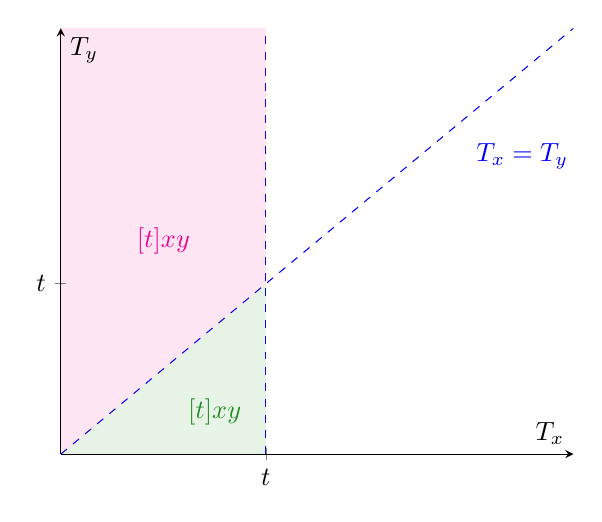
\begin{tikzpicture}[scale=0.95]
\begin{axis}[xmin=0, ymin=0, xmax=5, ymax=5,
xtick={2}, ytick={2}, xticklabels={\(t\)}, yticklabels={\(t\)}, axis lines=middle,
xlabel={\(T_x\)}, ylabel={\(T_y\)}]
\draw[blue, dashed] (0,0) -- (5,5);
\draw[blue, dashed] (2,0) -- (2,5);
\fill[ForestGreen, opacity=0.1] (0,0) -- (2,0) -- (2,2);
\fill[magenta, opacity=0.1] (0,0) -- (2,2) -- (2,5) -- (0,5) -- cycle;
\node[blue] () at (4.5,3.5) {\(T_x=T_y\)};
\node[ForestGreen] () at (1.5,0.5) {\(\qx[t]{\iitop{x}y}\)};
\node[magenta] () at (1,2.5) {\(\qx[t]{\itop{x}y}\)};
\end{axis}
\end{tikzpicture}
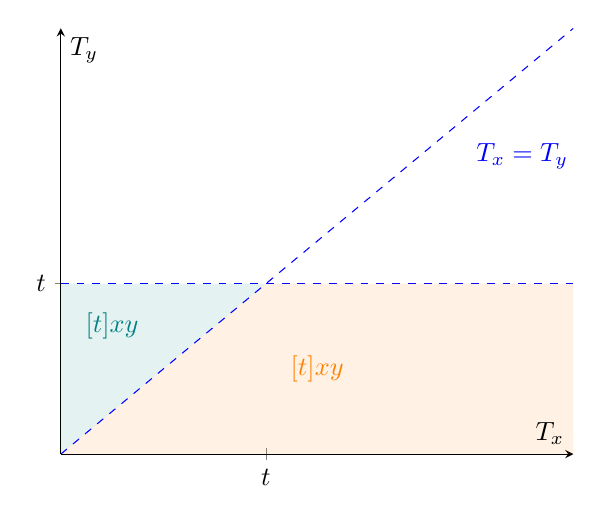
\begin{tikzpicture}[scale=0.95]
\begin{axis}[xmin=0, ymin=0, xmax=5, ymax=5,
xtick={2}, ytick={2}, xticklabels={\(t\)}, yticklabels={\(t\)}, axis lines=middle,
xlabel={\(T_x\)}, ylabel={\(T_y\)}]
\draw[blue, dashed] (0,2) -- (5,2);
\fill[teal, opacity=0.1] (0,0) -- (0,2) -- (2,2);
\fill[orange, opacity=0.1] (0,0) -- (2,2) -- (5,2) -- (5,0) -- cycle;
\draw[blue, dashed] (0,0) -- (5,5);
\node[blue] () at (4.5,3.5) {\(T_x=T_y\)};
\node[teal] () at (0.5,1.5) {\(\qx[t]{x\iitop{y}}\)};
\node[orange] () at (2.5,1) {\(\qx[t]{x\itop{y}}\)};
\end{axis}
\end{tikzpicture}
\end{center}
\begin{itemize}
\item \(\displaystyle \mgc{\qx[t]{\itop{x}y}}=\int_{0}^{t}\int_{u}^{\infty}f_{T_x,T_y}(u,v)\dd{v}\dd{u}\).
\item \(\displaystyle \gc{\qx[t]{\iitop{x}y}}=\int_{0}^{t}\int_{0}^{u}f_{T_x,T_y}(u,v)\dd{v}\dd{u}\).
\item \(\displaystyle \orc{\qx[t]{x\itop{y}}}=\int_{0}^{t}\int_{v}^{\infty}f_{T_x,T_y}(u,v)\dd{u}\dd{v}\).
\item \(\displaystyle \tec{\qx[t]{x\iitop{y}}}=\int_{0}^{t}\int_{0}^{v}f_{T_x,T_y}(u,v)\dd{u}\dd{v}\).
\end{itemize}
\begin{note}
\(f_{T_x,T_y}\) is the joint density function of \(T_x\) and \(T_y\).
\end{note}
\item \emph{Conditioning formulas:}
\begin{itemize}
\item \(\displaystyle \qx[t]{\itop{x}y}
=\int_{0}^{t}\underbrace{\prob{T_y>u|T_x=u}}_{\text{\((y)\) survives longer}}
\underbrace{\px[u]{x}\mu_{x+u}\dd{u}}_{\text{\((x)\) dies in \([u,u+\dd{u}]\)}}\).
\item \(\displaystyle \qx[t]{\iitop{x}y}=\int_{0}^{t}
\underbrace{\prob{T_y<u|T_x=u}}_{\text{\((y)\) died earlier}}
\underbrace{\px[u]{x}\mu_{x+u}\dd{u}}_{\text{\((x)\) dies in \([u,u+\dd{u}]\)}}
\).
\item \(\displaystyle \qx[t]{x\itop{y}}
=\int_{0}^{t}\underbrace{\prob{T_x>u|T_y=u}}_{\text{\((x)\) survives longer}}
\underbrace{\px[u]{y}\mu_{y+u}\dd{u}}_{\text{\((y)\) dies in \([u,u+\dd{u}]\)}}\).
\item \(\displaystyle \qx[t]{x\iitop{y}}=\int_{0}^{t}
\underbrace{\prob{T_x<u|T_y=u}}_{\text{\((x)\) died earlier}}
\underbrace{\px[u]{y}\mu_{y+u}\dd{u}}_{\text{\((y)\) dies in \([u,u+\dd{u}]\)}}
\).
\end{itemize}
\begin{pf}
(Sketch) Consider the first formula as an example. We can use the law of
total expectation as follows:
\begin{align*}
\qx[t]{\itop{x}y}
&=\prob{\vc{T_x}<T_y\cap \vc{T_x}\le t} \\
&=\expv{\indicset{\vc{T_x}<T_y}\indicset{\vc{T_x}\le t}} \\
&=\expv{\expv{\indicset{\vc{T_x}<T_y}\indicset{\vc{T_x}\le t}|\vc{T_x}}} \\
&=\expv{\expv{\indicset{\vc{T_x}<T_y}|\vc{T_x}}\indicset{\vc{T_x}\le t}}.
\end{align*}
Now define \(g(\vc{T_x}):=\expv{\indicset{\vc{T_x}<T_y}|\vc{T_x}}\), and then
we have
\[
\qx[t]{\itop{x}y}
=\int_{0}^{t}g(\vc{u})\underbrace{\px[u]{x}\mu_{x+u}}_{f_{x}(u)}\dd{u}
=\int_{0}^{t}\underbrace{\expv{\indicset{\vc{T_x}<T_y}|\vc{T_x=u}}}
_{\mathclap{=\expv{\indicset{u<T_y}|T_x=u}:=\prob{T_y>u|T_x=u}}}
\px[u]{x}\mu_{x+u}\dd{u}.
\]
\end{pf}
\item \emph{Relationships:} Assume that simultaneous death is impossible, i.e.,
\(\mu_{x+t:y+t}^{03}\equiv 0\), so that \(\prob{T_x=T_y}=0\).
\begin{itemize}
\item
\[
\underbrace{\mgc{\qx[t]{\itop{x}y}}}_{\text{\((x)\) dies 1st}}
+\underbrace{\gc{\qx[t]{\iitop{x}y}}}_{\text{\((x)\) dies 2nd}}
=\underbrace{\qx[t]{x}}_{\text{\((x)\) dies}}.
\]
\item
\[
\underbrace{\orc{\qx[t]{x\itop{y}}}}_{\text{\((y)\) dies 1st}}
+\underbrace{\tec{\qx[t]{x\iitop{y}}}}_{\text{\((y)\) dies 2nd}}
=\underbrace{\qx[t]{x}}_{\text{\((y)\) dies}}.
\]
\item \[
\underbrace{\mgc{\qx[t]{\itop{x}y}}}_{\text{\((x)\) dies 1st}}
+\underbrace{\orc{\qx[t]{x\itop{y}}}}_{\text{\((y)\) dies 1st}}
=\underbrace{\qx[t]{xy}}_{\text{1st death}}.
\]
\item \[
\underbrace{\gc{\qx[t]{\iitop{x}y}}}_{\text{\((x)\) dies 2nd}}
+\underbrace{\tec{\qx[t]{x\iitop{y}}}}_{\text{\((y)\) dies 2nd}}
=\underbrace{\qx[t]{\overline{xy}}}_{\text{2nd death}}.
\]
\end{itemize}
\begin{center}
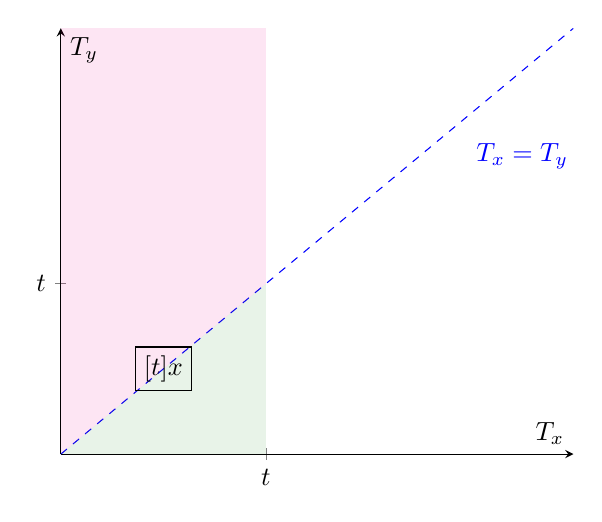
\begin{tikzpicture}[scale=0.95]
\begin{axis}[xmin=0, ymin=0, xmax=5, ymax=5,
xtick={2}, ytick={2}, xticklabels={\(t\)}, yticklabels={\(t\)}, axis lines=middle,
xlabel={\(T_x\)}, ylabel={\(T_y\)}]
\draw[blue, dashed] (0,0) -- (5,5);
\fill[ForestGreen, opacity=0.1] (0,0) -- (2,0) -- (2,2);
\fill[magenta, opacity=0.1] (0,0) -- (2,2) -- (2,5) -- (0,5) -- cycle;
\node[blue] () at (4.5,3.5) {\(T_x=T_y\)};
\node[draw] () at (1,1) {\(\qx[t]{x}\)};
\end{axis}
\end{tikzpicture}
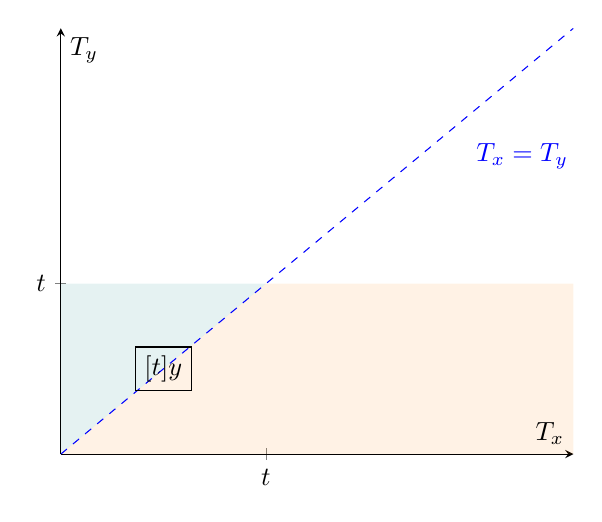
\begin{tikzpicture}[scale=0.95]
\begin{axis}[xmin=0, ymin=0, xmax=5, ymax=5,
xtick={2}, ytick={2}, xticklabels={\(t\)}, yticklabels={\(t\)}, axis lines=middle,
xlabel={\(T_x\)}, ylabel={\(T_y\)}]
\fill[teal, opacity=0.1] (0,0) -- (0,2) -- (2,2);
\fill[orange, opacity=0.1] (0,0) -- (2,2) -- (5,2) -- (5,0) -- cycle;
\draw[blue, dashed] (0,0) -- (5,5);
\node[blue] () at (4.5,3.5) {\(T_x=T_y\)};
\node[draw] () at (1,1) {\(\qx[t]{y}\)};
\end{axis}
\end{tikzpicture}
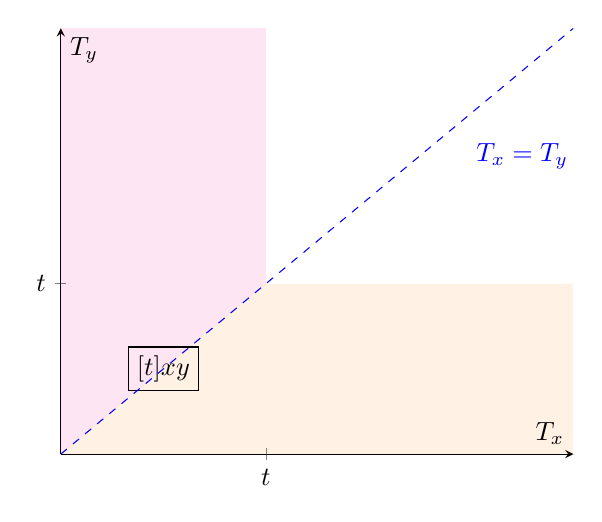
\begin{tikzpicture}[scale=0.95]
\begin{axis}[xmin=0, ymin=0, xmax=5, ymax=5,
xtick={2}, ytick={2}, xticklabels={\(t\)}, yticklabels={\(t\)}, axis lines=middle,
xlabel={\(T_x\)}, ylabel={\(T_y\)}]
\fill[orange, opacity=0.1] (0,0) -- (2,2) -- (5,2) -- (5,0) -- cycle;
\fill[magenta, opacity=0.1] (0,0) -- (2,2) -- (2,5) -- (0,5) -- cycle;
\node[draw] () at (1,1) {\(\qx[t]{xy}\)};
\draw[blue, dashed] (0,0) -- (5,5);
\node[blue] () at (4.5,3.5) {\(T_x=T_y\)};
\end{axis}
\end{tikzpicture}
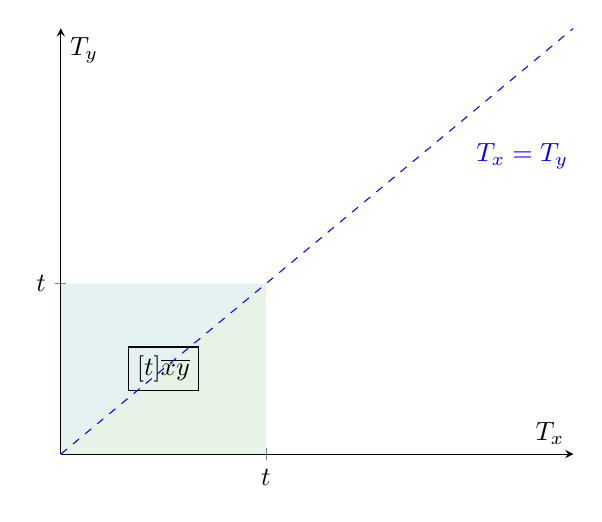
\begin{tikzpicture}[scale=0.95]
\begin{axis}[xmin=0, ymin=0, xmax=5, ymax=5,
xtick={2}, ytick={2}, xticklabels={\(t\)}, yticklabels={\(t\)}, axis lines=middle,
xlabel={\(T_x\)}, ylabel={\(T_y\)}]
\fill[ForestGreen, opacity=0.1] (0,0) -- (2,0) -- (2,2);
\fill[teal, opacity=0.1] (0,0) -- (0,2) -- (2,2);
\node[draw] () at (1,1) {\(\qx[t]{\overline{xy}}\)};
\draw[blue, dashed] (0,0) -- (5,5);
\node[blue] () at (4.5,3.5) {\(T_x=T_y\)};
\end{axis}
\end{tikzpicture}
\end{center}
\end{enumerate}
\end{enumerate}
\item \textbf{Specialized probability calculation formulas based on multiple
state model.} Several more formulas for probabilities about order of death can
be obtained by viewing them from a multiple state model perspective, and
specializing the general probability calculation formula in
\labelcref{it:gen-prob-fmla}:
\begin{itemize}
\item \(\displaystyle \qx[t]{\itop{x}y}=\int_{0}^{t}\px[u]{xy}[00]\blc{\mu_{x+u:y+u}^{02}\dd{u}}
\rc{\;\ne \px[t]{xy}[02]}\) \warn{}.
\item \(\displaystyle \qx[t]{\iitop{x}y}=\int_{0}^{t}\mgc{\px[u]{xy}[01]}\orc{\mu_{x+u:y+u}^{13}\dd{u}}
\rc{\;\ne \px[t]{xy}[03]\text{ or }\px[t]{xy}[13]}\) \warn{}.
\item \(\displaystyle \qx[t]{x\itop{y}}=\int_{0}^{t}\px[u]{xy}[00]\mgc{\mu_{x+u:y+u}^{01}\dd{u}}
\rc{\;\ne \px[t]{xy}[01]}\) \warn{}.
\item \(\displaystyle \qx[t]{x\iitop{y}}=\int_{0}^{t}\blc{\px[u]{xy}[02]}\vc{\mu_{x+u:y+u}^{23}\dd{u}}
\rc{\;\ne \px[t]{xy}[03]\text{ or }\px[t]{xy}[23]}\) \warn{}.
\end{itemize}
\begin{center}
\begin{tikzpicture}
\node[draw, minimum width=3cm, minimum height=1.5cm] () at (0,0) {Both alive (0)};
\node[draw, minimum width=3cm, minimum height=1.5cm] () at (7,0) {Only \((x)\) alive (1)};
\node[draw, minimum width=3cm, minimum height=1.5cm] () at (0,-3) {Only \((y)\) alive (2)};
\node[draw, minimum width=3cm, minimum height=1.5cm] () at (7,-3) {Both dead (3)};
\draw[-Latex, magenta] (1.5,0) --node[midway, above]{\((y)\) dies 1st} (5.5,0);
\draw[-Latex, orange] (7,-0.75) --node[midway, right]{\((x)\) dies 2nd} (7,-2.25);
\draw[-Latex, blue] (0,-0.75) --node[midway, left]{\((x)\) dies 1st} (0,-2.25);
\draw[-Latex, violet] (1.5,-3) --node[midway, below]{\((y)\) dies 2nd} (5.5,-3);
\draw[-Latex] (1.5,-0.75) --node[midway]{simultaneous death} (5.5,-2.25);
\end{tikzpicture}
\end{center}
\begin{note}
When simultaneous death occurs, \((x)\) dies \underline{neither} before
\underline{nor} after \((y)\). (We are using ``before'' and ``after'' in the
strict sense.)
\end{note}

Although the equation \(\qx[t]{\itop{x}y}=\px[t]{xy}[02]\) may appear to be
intuitively appealing, it is actually wrong \warn{}. After thinking more
carefully, we can observe that the latter (\(\px[t]{xy}[02]\)) requires the
system to be in state 2 \faIcon{at} time \(t\), while the former
(\(\qx[t]{\itop{x}y}\)) does not: We just need to have a transition from state
0 to state 2 within \(t\) years, and we do not care about what happens next
(staying in state 2 or transiting further to state 3 are both fine). In fact,
we have \(\mgc{\qx[t]{\itop{x}y}}=\underbrace{\tec{\qx[t]{x\iitop{y}}}}_{\text{go to state 3 next}}
+\underbrace{\orc{\px[t]{xy}[02]}}_{\text{stay in state 2}}\) instead,
which can be intuitively understood based on the following picture:
\begin{center}
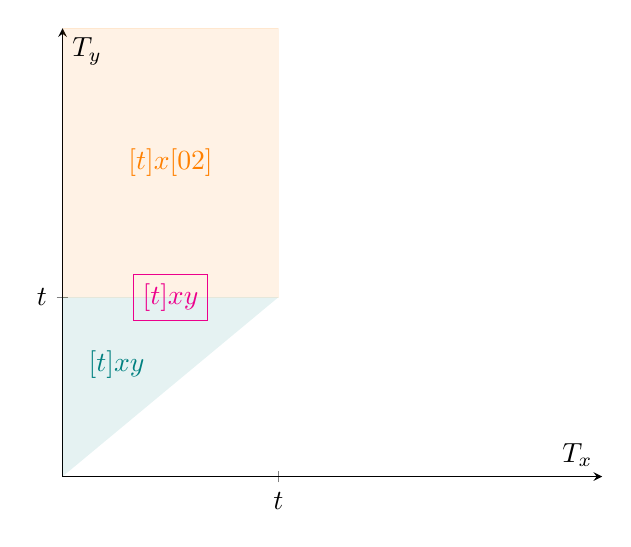
\begin{tikzpicture}
\begin{axis}[xmin=0, ymin=0, xmax=5, ymax=5,
xtick={2}, ytick={2}, xticklabels={\(t\)}, yticklabels={\(t\)}, axis lines=middle,
xlabel={\(T_x\)}, ylabel={\(T_y\)}]
\draw[fill, orange, opacity=0.1] (0,2) rectangle (2,5);
\node[orange] () at (1,3.5) {\(\px[t]{x}[02]\)};
\fill[teal, opacity=0.1] (0,0) -- (0,2) -- (2,2);
\node[teal] () at (0.5,1.25) {\(\qx[t]{x\iitop{y}}\)};
\node[magenta, draw] () at (1,2) {\(\qx[t]{\itop{x}y}\)};
\end{axis}
\end{tikzpicture}
\end{center}
\item\label{it:independent-life-fmlas} \textbf{Independent model.} Many
formulas discussed previously can be simplified a lot when we assume
\emph{independent lifetimes} in the multiple life model (perhaps not so
realistic in practice). Of course, we can characterize the independent
lifetimes assumption by ``\(T_x\) and \(T_y\) are independent''. This is a
natural characterization based on the random variable approach. Another less
natural but equivalent characterization based on the multiple state model
approach is as follows:
\begin{itemize}
\item \emph{(\((y)\)'s mortality does not depend on \((x)\)'s status)} \(\mu_{x+t:y+t}^{01}=\mu_{y+t}^{23}=\mu_{y+t}^{f}\)
\item \emph{(\((x)\)'s mortality does not depend on \((y)\)'s status)} \(\mu_{x+t:y+t}^{02}=\mu_{x+t}^{13}=\mu_{x+t}^{m}\)
\item \emph{(no simultaneous death)} \(\mu_{x+t:y+t}^{03}=0\)
\end{itemize}
\begin{note}
By treating the lives \((x)\) and \((y)\) as ``husband (male)'' and ``wife
(female)'', we can understand why the notations \(\mu_{x+t}^{\vc{m}}\) and
\(\mu_{y+t}^{\vc{f}}\) are used.
\end{note}
\begin{center}
\begin{tikzpicture}
\node[draw, minimum width=3cm, minimum height=1.5cm] () at (0,0) {Both alive (0)};
\node[draw, minimum width=3cm, minimum height=1.5cm] () at (7,0) {Only \((x)\) alive (1)};
\node[draw, minimum width=3cm, minimum height=1.5cm] () at (0,-3) {Only \((y)\) alive (2)};
\node[draw, minimum width=3cm, minimum height=1.5cm] () at (7,-3) {Both dead (3)};
\draw[-Latex] (1.5,0) --node[midway, above]{\(\mu_{y+t}^{f}\)} (5.5,0);
\draw[-Latex] (7,-0.75) --node[midway, right]{\(\mu_{x+t}^{m}\)} (7,-2.25);
\draw[-Latex] (0,-0.75) --node[midway, left]{\(\mu_{x+t}^{m}\)} (0,-2.25);
\draw[-Latex] (1.5,-3) --node[midway, below]{\(\mu_{y+t}^{f}\)} (5.5,-3);
\end{tikzpicture}
\end{center}
Under this independence assumption, we have
\[
\boxed{\px[t]{xy}=\px[t]{x}\cdot \px[t]{y}}
\qqtext{and}
\boxed{\qx[t]{\overline{xy}}=\qx[t]{x}\cdot \qx[t]{y}}.
\]
\begin{warning}
We do NOT have ``\(\qx[t]{xy}=\qx[t]{x}\cdot \qx[t]{y}\)'' and
``\(\px[t]{\overline{xy}}=\px[t]{x}\cdot \px[t]{y}\)''! For joint-life status,
we can only ``split \(p\)''; For last-survivor status, we can only ``split
\(q\)''.
\end{warning}

These allow us to simplify many formulas discussed before.

Of course, we can extend this assumption to the case with 3 or more lives, but
in such case we often only use the characterization based on random variable
approach, due to the complexity of multiple state model when handling 3 or more
lives.
\end{enumerate}
\subsection{Insurance and Annuity EPV Calculations}
\label{subsect:mult-life-insur-annu-epv}
\begin{enumerate}
\item After completing the (lengthy!) discussions on probabilistic calculations
for multiple life model, it is time to apply the concepts and formulas learnt
there to calculate EPVs (and related quantities like variances of PVRVs) for
various kinds of insurance and annuity products issued to multiple lives
(ultimately, the existence of these products is the reason why the topic of
multiple life model appears in STAT3909!).

\item Certainly, concepts and formulas from \Cref{sect:mult-state-models} can
be applied here to help us calculating the EPVs. However, some products to be
discussed here have special features that cannot be described using just the
terminologies in \Cref{subsect:mult-state-insur-ann-epv}, which forces us to
develop some new concepts and formulas to deal with those products. In
particular, as we know from \Cref{subsect:mult-life-prob-calc}, in multiple
life model we have two kinds of ``special lives'': joint-life and last-survivor
statuses. One natural strategy is then to ``revisit'' topics about life
insurance and life annuity from STAT3901 for these ``special lives'', which can
yield numerous formulas and tools for analyzing the products.

So, as you can expect after reading the paragraph above,
\Cref{subsect:mult-life-insur-annu-epv} will again be rather
lengthy...\footnote{It is quite normal to feel overwhelmed
\faIcon[regular]{tired} by the \emph{sheer} amount of terms and formulas you
have seen so far. (If you do \emph{not} feel that, you would probably get A+ in
STAT3909 easily \faIcon[regular]{laugh-wink}.) \Cref{sect:mult-life-models} is
indeed a rather challenging part in STAT3909, and it does take time to digest
such a large amount of content here.} Nonetheless, the good
\faIcon[regular]{thumbs-up} news is that the versatile \emph{general EPV
calculation formula} will continue to be of great use.

\subsubsection*{Revisiting Insurance and Annuity Topics for Joint-Life and
Last-Survivor Statuses}
\item Instead of revisiting the \emph{enormous} amount of life insurance and
annuity formulas from STAT3901 \emph{one by one}, here we will just study some
key points and formulas (and also some pitfalls \warn{}), because many formulas
there are just specialized versions of the \emph{general EPV calculation
formula}.

\item \textbf{Insurances.}
\begin{enumerate}[label={(\arabic*)}]
\item \emph{Notations:} Insurance notations from STAT3901 still apply for
joint-life and last-survivor statuses and carry the same meaning (with the
future lifetime random variable \(T\) being the ``lifetime'' of one of these
``special lives''); We just need to change the age ``\(x\)'' in the notation to
``\(xy\)'' or ``\(\overline{xy}\)''. The only special thing is that for term
life insurance notation, we would add a hat on top of \(xy\) (joint-life status
only) to make the notations better-looking.

Examples:
\[
\Ax{x}\to\begin{cases}
\Ax{xy} \\
\Ax{\overline{xy}}
\end{cases}\quad
\Ax{\termxn}\to
\begin{cases}
\Ax{\itop{\rc{\widehat{xy}}}:\angl{n}} \\
\Ax{\itop{\overline{xy}}:\angl{n}}
\end{cases}\quad
\Ax{\endowxn}\to
\begin{cases}
\Ax{xy:\angl{n}} \\
\Ax{\overline{xy}:\angl{n}}
\end{cases}\quad
\Ax{\pureendowxn}\to
\begin{cases}
\Ax{xy:\itop{\angl{n}}} \\
\Ax{\overline{xy}:\itop{\angl{n}}}
\end{cases}\quad
\Ex[n]{x}\to
\begin{cases}
\Ex[n]{xy} \\
\Ex[n]{\overline{xy}}
\end{cases}
\]
\item \emph{Formulas (examples):}
\begin{enumerate}[label={(\roman*)}]
\item \emph{Specialized EPV calculation formulas:}
\begin{align*}
\Ax{xy}=\sum_{k=0}^{\infty}\vc{v^{k+1}}\mgc{\px[k]{xy}\qx[]{x+k:y+k}}
&\qquad\Ax*{xy}=\int_{0}^{\infty}\vc{e^{-\delta t}}\mgc{\px[t]{xy}
\underbrace{\mu_{x+t:y+t}}_{\text{or \(\mu_{xy}(t)\)}}\dd{t}} \\
\Ax{\overline{xy}}=\sum_{k=0}^{\infty}
\vc{v^{k+1}}\rc{\xcancel{\px[k]{xy}\qx[]{\overline{x+k:y+k}}}}
\mgc{\px[k|]{\overline{xy}}}
&\qquad\Ax*{\overline{xy}}=\int_{0}^{\infty}\vc{e^{-\delta t}}\mgc{\px[t]{\overline{xy}}
\rc{\xcancel{\mu_{\overline{x+t:y+t}}}}\mu_{\overline{xy}}(t)
\dd{t}} \\
\end{align*}
\item \emph{Variance formulas:}
\[
\vari{\text{PVRV}}=\Ax[][2]{\square}-\Ax{\square}^{2}
\]
where \(\square\) is the appropriate symbol for the insurance and status being
considered (e.g., \(xy\!:\!\angl{n}\) for an \(n\)-year endowment insurance
``issued to'' \((xy)\)). Change \(\Ax{}\to\Ax*{}\) for the continuous case
(except pure endowment).

\item \emph{Relationships:} 
\begin{itemize}
\item \emph{(\(\text{endowment}=\text{term}+\text{pure endowment}\))}
\[
\Ax{\square:\angl{n}}=\Ax{\itop{\square}:\angl{n}}+\Ax{\square:\itop{\angl{n}}}.
\]
\item \emph{(\(\text{deferred}=\text{WL}-\text{term}\))}
\[
\Ax[n|]{\square}=\Ax{\itop{\square}}-\Ax{\itop{\square}:\angl{n}}.
\]

\item \emph{(discounted EPV formula for \textbf{joint-life status})}
\[
\Ax[n|]{xy}=\Ex[n]{xy}\Ax{x+n:y+n}.
\]
\begin{warning}
We do NOT have
``\(\Ax[n|]{\overline{xy}}=\Ex[n]{\overline{xy}}\Ax{\overline{x+t:y+t}}\)''!
\end{warning}
\item \emph{(second moment of pure endowment)}
\[
\Ex[n]{\square}=v^{n}\Ex[n]{\square}.
\]
\end{itemize}
\begin{remark}
\item \(\square=xy\text{ or }\overline{xy}\).
\item Change \(\Ax{}\to\Ax*{}\) for the continuous case.
\item Use the notation \(\Ax{\itop{\rc{\widehat{xy}}}:\angl{n}}\) instead of
\(\Ax{\itop{xy}:\angl{n}}\).
\end{remark}
\end{enumerate}
\end{enumerate}
\item \textbf{Annuities.}
\begin{enumerate}[label={(\arabic*)}]
\item \emph{Notations:} Annuity notations from STAT3901 still apply for
joint-life and last-survivor statuses; Again we just need to change the age
``\(x\)'' in the notation to ``\(xy\)'' or ``\(\overline{xy}\)''.

Examples:
\[
\ax**{x}\to\begin{cases}
\ax**{xy} \\
\ax**{\overline{xy}}
\end{cases}\quad
\ax**{\endowxn}\to
\begin{cases}
\ax**{xy:\angl{n}} \\
\ax**{\overline{xy}:\angl{n}}
\end{cases}\quad
\ax**[n|]{x}\to
\begin{cases}
\ax**[n|]{xy} \\
\ax**[n|]{\overline{xy}}
\end{cases}\quad
\ax**{\overline{\endowxn}}\to
\begin{cases}
\ax**{\overline{xy:\angl{n}}} \\
\ax**{\overline{\overline{xy}:\angl{n}}}\text{\quad\faIcon{arrow-left} look carefully \warn{}}
\end{cases}
\]
\item \emph{Formulas (examples):}
\begin{enumerate}[label={(\roman*)}]
\item \emph{Specialized EPV calculation formulas:}
\begin{align*}
\ax**{xy}=\sum_{k=0}^{\infty}\vc{v^k}\mgc{\px[k]{xy}}
&\qquad\ax*{xy}=\int_{0}^{\infty}\vc{e^{-\delta t}}\mgc{\px[t]{xy}}\brc{\dd{t}} \\
\ax**{\overline{xy}}=\sum_{k=0}^{\infty}\vc{v^k}\mgc{\px[k]{\overline{xy}}}
&\qquad\ax*{\overline{xy}}=\int_{0}^{\infty}\vc{e^{-\delta t}}\mgc{\px[t]{\overline{xy}}}\brc{\dd{t}}
\end{align*}
\item \emph{Variance formulas (for WL or temporary life annuity):}
\[
\vari{\text{PVRV}}=\frac{\Ax[][2]{\square}-\Ax{\square}^{2}}{d^2}
\]
where \(\square=\text{\(xy\), \(\overline{xy}\), \(xy\!:\!\angl{n}\), or
\(\overline{xy}\!:\!\angl{n}\)} \). For the continuous case, change
\(\Ax{}\to\Ax*{}\) and \(d\to\delta\).
\item \emph{Relationships:}
\begin{itemize}
\item \emph{(\(\text{deferred}=\text{WL}-\text{temporary}\))}
\[
\ax**[n|]{\square}=\ax**{\square}-\ax**{\square:\angl{n}}
\]
\item \emph{(\(\text{guaranteed}=\text{certain}+\text{deferred}\))}
\[
\ax**{\overline{\square:\angl{n}}}=\ax**{\angl{n}}+\ax**[n|]{\square}
\]
\item \emph{(discounted EPV formula for \textbf{joint-life status})}

\[
\ax**[n|]{xy}=\Ex[n]{xy}\ax**{x+n:y+n}
\]

\begin{warning}
We do NOT have
``\(\ax**[n|]{\overline{xy}}=\Ex[n]{\overline{xy}}\ax**{\overline{x+n:y+n}}\)''!
\end{warning}
\end{itemize}
\begin{remark}
\item \(\square=xy\text{ or }\overline{xy}\).
\item Change \(\ax**{}\to\ax*{}\) for the continuous case.
\end{remark}
\end{enumerate}
\end{enumerate}
\item \textbf{Recursions for insurance and annuity EPVs.} Regarding
\emph{recursions}, one important thing to bear in mind is that we do NOT have
any recursive formula for last-survivor status \warn{}, due to the breakdown of
the ``factorization formula for \(p\)'' (which is foundational to recursions)
for last-survivor status. On the other hand, we do have recursive formulas
available for joint-life status, which can be obtained by adapting the
recursive formulas from STAT3901:
\begin{itemize}
\item \emph{Whole life insurance:}
\begin{itemize}
\item \emph{(discrete)}
\(\Ax{xy}=\Ax{\itop{\widehat{xy}}:\angl{n}}+\Ex[n]{xy}\Ax{x+n:y+n}
\overset{(n=1)}{=}v\qx[]{xy}+v\px[]{xy}\Ax{x+1:y+1}\).
\item \emph{(continuous)} \(\Ax*{xy}=\Ax*{\itop{\widehat{xy}}:\angl{n}}+\Ex[n]{xy}\Ax*{x+n:y+n}\).
\end{itemize}
\item \emph{Term life insurance:}
\begin{itemize}
\item \emph{(discrete)} \(\Ax{\itop{\widehat{xy}}:\angl{n}}\overset{(m\le n)}{=}\Ax{\itop{\widehat{xy}}:\angl{m}}
+\Ex[m]{xy}\Ax{\itop{\widehat{x+m:y+m}}:\angl{n-m}}
\overset{(m=1)}{=}v\qx[]{xy}+v\px[]{xy}\Ax{\itop{\widehat{x+1:y+1}}:\angl{n-1}}\).
\item \emph{(continuous)} \(\Ax*{\itop{\widehat{xy}}:\angl{n}}
\overset{(m\le n)}{=}\Ax*{\itop{\widehat{xy}}:\angl{m}}
+\Ex[m]{xy}\Ax*{\itop{\widehat{x+m:y+m}}:\angl{n-m}}\).
\end{itemize}

\item \emph{Endowment insurance:}
\begin{itemize}
\item \emph{(discrete)} \(\Ax{xy:\angl{n}}\overset{(m\le n)}{=}\Ax{\itop{\widehat{xy}}:\angl{m}}
+\Ex[m]{xy}\Ax{x+m:y+m:\angl{n-m}}\overset{(m=1)}{=}v\qx[]{xy}+v\px[]{xy}\Ax{x+1:y+1:\angl{n-1}}\).
\item \emph{(continuous)} \(\Ax*{\itop{\widehat{xy}}:\angl{n}}
\overset{(m\le n)}{=}\Ax*{\itop{\widehat{xy}}:\angl{m}}+\Ex[m]{xy}\Ax*{x+m:y+m:\angl{n-m}}\).
\end{itemize}
\end{itemize}
\begin{itemize}
\item \emph{Whole life annuity:}
\begin{itemize}
\item \emph{(discrete, due)} \(\ax**{xy}=\ax**{xy:\angl{n}}+\Ex[n]{xy}\ax**{x+n:y+n}
\overset{(n=1)}{=}\vc{1}+v\px{xy}\ax**{x+1:y+1}\).
\item \emph{(continuous)} \(\ax*{xy}=\ax*{xy:\angl{n}}+\Ex[n]{xy}\ax*{x+n:y+n}\).
\end{itemize}
\item \emph{Temporary life annuity:}
\begin{itemize}
\item \emph{(discrete, due)} \(\ax**{xy:\angl{n}}\overset{(m\le n)}{=}\ax**{xy:\angl{m}}+\Ex[m]{xy}\ax**{x+m:y+m:\angl{n-m}}
\overset{(m=1)}{=}\vc{1}+v\px{xy}\ax**{x+1:y+1:\angl{n-1}}\).
\item \emph{(continuous)} \(\ax*{xy:\angl{n}}=\ax*{xy:\angl{m}}+\Ex[m]{xy}\ax*{x+m:y+m:\angl{n-m}}\).
\end{itemize}
\end{itemize}
\item \label{it:cov-wl-pvrvs} \textbf{Covariance between WL PVRVs.} With the
presence of \emph{two} random variables \(T_x\) and \(T_y\) in multiple life
model, \emph{covariance} between PVRVs would be of more interest. Recall the
covariance formula discussed previously in \labelcref{it:fail-time-moments}:
\[
\cov{T_{xy}}{T_{\overline{xy}}}=\cov{T_x}{T_y}+(\eringx{x}-\eringx{xy})(\eringx{y}-\eringx{xy}).
\]
For whole life insurance PVRV, we have a formula having similar form:
\[
\cov{v^{T_{xy}}}{v^{T_{\overline{xy}}}}=\boxed{\cov{v^{T_x}}{v^{T_y}}+(\Ax*{x}-\Ax*{xy})(\Ax*{y}-\Ax*{xy})},
\]
which can be proved in a similar way as the proof for the covariance formula
above, utilizing the identity \(v^{T_{xy}}v^{T_{\overline{xy}}}\equiv
v^{T_{x}}v^{T_{y}}\) (try it!).

\item \label{it:jl-ls-epv-sum} \textbf{\(\text{Joint-life}+\text{Last-survivor}=\text{Individual sum}\).} 
In \Cref{subsect:mult-life-prob-calc}, we have seen this type of relationship
for ``\(\px[t]{\square}\)'', ``\(\qx[t]{\square}\)'', ``\(e_{\square}\)'',
``\(\eringx{\square}\)'', and \(f_{\square}(t)\) (density function).  Using a
similar argument, we can derive relationships of this kind for insurance and
annuity EPVs:
\begin{itemize}
\item \emph{Insurance EPV:}
\[
\Ax{xy}+\Ax{\overline{xy}}=\Ax{x}+\Ax{y}.
\]
Possible variations:
\begin{itemize}
\item \emph{(continuous)} \(\Ax{}\to\Ax*{}\)
\item \emph{(term life)} \(\text{WL subscript}\to\text{term life subscript}\)
\item \emph{(endowment)} \(\text{WL subscript}\to\text{endowment subscript}\)
\item \emph{(pure endowment)} \(\Ax{xy}\to\Ex[n]{xy}\), etc.
\end{itemize}
\item \emph{Annuity EPV:}
\[
\ax**{xy}+\ax**{\overline{xy}}=\ax**{x}+\ax**{y}.
\]

Possible variations:
\begin{itemize}
\item \emph{(continuous)} \(\ax**{}\to\ax*{}\)
\item \emph{(temporary life)} \(\text{WL subscript}\to\text{temporary life subscript}\)
\end{itemize}
\end{itemize}

\subsubsection*{Connections with multiple state model}
\item Apart from developing the formulas based on the random variable approach
like what we have done above, we can also obtain some formulas by viewing the
insurance and annuity products here as \emph{state-contingent} products, and
applying the formulas developed in \Cref{subsect:mult-state-insur-ann-epv}.
(Recall how we revise the multiple state EPV notations from
\labelcref{it:revised-mult-state-notations}.)

\item \textbf{Insurances and annuities for joint-life status.}
\begin{center}
\begin{tikzpicture}
\node[draw, minimum width=3cm, minimum height=1.5cm] () at (0,0) {Both alive (0)};
\node[draw, minimum width=3cm, minimum height=1.5cm] () at (7,0) {Only \((x)\) alive (1)};
\node[draw, minimum width=3cm, minimum height=1.5cm] () at (0,-3) {Only \((y)\) alive (2)};
\node[draw, minimum width=3cm, minimum height=1.5cm] () at (7,-3) {Both dead (3)};
\draw[-Latex, red] (1.5,0) --node[midway, above]{\((xy)\) ``dies''} (5.5,0);
\draw[-Latex] (7,-0.75) -- (7,-2.25);
\draw[-Latex, red] (0,-0.75) --node[midway, left]{\((xy)\) ``dies''} (0,-2.25);
\draw[-Latex] (1.5,-3) -- (5.5,-3);
\draw[-Latex, red] (1.5,-0.75) --node[midway, below=0.3cm]{\((xy)\) ``dies''} (5.5,-2.25);
\end{tikzpicture}
\end{center}
Based on this picture and the general EPV calculation formula, we can obtain
the following formulas.
\begin{note}
In some formulas below, we need to assume that it is impossible to directly
transit from state 0 to state 3 (simultaneous death, or \defn{common shock}).
We will abbreviate this assumption as ``NCS'' (\underline{n}o
\underline{c}ommon \underline{s}hock).
\end{note}
\begin{center}
\begin{tabular}{lll}
\toprule
Type&Discrete&Continuous \\
\midrule
WL insurance&
\makecell[l]{
\(\displaystyle \Ax{xy}\overset{\text{(NCS)}}{=}
\Ax{xy}[01]+\Ax{xy}[02]\) \\
\(\displaystyle \rc{\ne}\sum_{t=0}^{\infty}\vc{v^{t+1}}\mgc{\px[t]{xy}[00]
\px{x+t:y+t}[0\bullet]}\text{ without NCS}\)
}
&
\makecell[l]{
\(\displaystyle \Ax*{xy}
=\overbrace{\int_{0}^{\infty}\vc{e^{-\delta t}}
\mgc{\px[t]{xy}[00]\mu_{x+t:y+t}^{0\bullet}\dd{t}}}
^{\text{NOT \(\Ax*{x}[01]+\Ax*{x}[02]+\Ax*{x}[03]\) \warn{}}}\) \\
\(\displaystyle
\overset{\text{(NCS)}}{=}
\Ax*{xy}[01]+\Ax*{xy}[02]
\)
} \\
\midrule
WL annuity&
(due) \(\displaystyle \ax**{xy}=\ax**{xy}[00]\)
& \(\displaystyle \ax*{xy}=\ax*{xy}[00]\)\\
\midrule
\(n\)-year term life insurance&
\(\displaystyle \Ax{\itop{\widehat{xy}}:\angl{n}}\overset{\text{(NCS)}}{=}
\Ax{xy:\angl{n}}[01]+\Ax{xy:\angl{n}}[02]\)
&
\makecell[l]{
\(\displaystyle \Ax*{\itop{\widehat{xy}}:\angl{n}}
=\int_{0}^{\blc{n}}\vc{e^{-\delta t}}
\mgc{\px[t]{xy}[00]\mu_{x+t:y+t}^{0\bullet}\dd{t}}\) \\
\(\displaystyle
\overset{\text{(NCS)}}{=}
\Ax*{xy:\angl{n}}[01]+\Ax*{xy:\angl{n}}[02]
\)
}\\
\midrule
\(n\)-year temporary annuity&
(due) \(\displaystyle \ax**{xy:\angl{n}}=\ax**{xy:\angl{n}}[00]\)
& \(\displaystyle \ax*{xy:\angl{n}}=\ax*{xy:\angl{n}}[00]\)\\
\bottomrule
\end{tabular}
\end{center}
\item \textbf{Insurances and annuities for last-survivor status.}
\begin{center}
\begin{tikzpicture}
\node[draw, minimum width=3cm, minimum height=1.5cm] () at (0,0) {Both alive (0)};
\node[draw, minimum width=3cm, minimum height=1.5cm] () at (7,0) {Only \((x)\) alive (1)};
\node[draw, minimum width=3cm, minimum height=1.5cm] () at (0,-3) {Only \((y)\) alive (2)};
\node[draw, minimum width=3cm, minimum height=1.5cm] () at (7,-3) {Both dead (3)};
\draw[-Latex] (1.5,0) -- (5.5,0);
\draw[-Latex] (0,-0.75) -- (0,-2.25);
\draw[-Latex, red] (7,-0.75) --node[midway, right]{\((\overline{xy})\) ``dies''} (7,-2.25);
\draw[-Latex, red] (1.5,-3) --node[midway, below]{\((\overline{xy})\) ``dies''} (5.5,-3);
\draw[-Latex, red] (1.5,-0.75) --node[midway, below=0.3cm]{\((\overline{xy})\) ``dies''} (5.5,-2.25);
\end{tikzpicture}
\end{center}
Based on this picture and the general EPV calculation formula, we can obtain
the following formulas.
\begin{center}
\begin{tabular}{lll}
\toprule
Type&Discrete&Continuous \\
\midrule
WL insurance&
\(\Ax{\overline{xy}}=
\Ax{xy}[03]\text{ (not ``\(\Ax{\overline{xy}}[03]\)''!)}\)
&\(\Ax*{xy}=\Ax*{xy}[03]\) \\
\midrule
WL annuity&
(due) \(\displaystyle \ax**{\overline{xy}}
=\ax**{xy}[00]+\ax**{xy}[01]+\ax**{xy}[02]\)
& \(\displaystyle \ax*{\overline{xy}}
=\ax*{xy}[00]+\ax*{xy}[01]+\ax*{xy}[02]
\)\\
\midrule
\(n\)-year term life insurance&
\(\Ax{\itop{\overline{xy}}:\angl{n}}=\Ax{xy:\angl{n}}[03]\)
& \(\Ax*{\itop{\overline{xy}}:\angl{n}}=\Ax*{xy:\angl{n}}[03]\)
\\
\midrule
\(n\)-year temporary annuity&
(due) \(\displaystyle \ax**{\overline{xy}:\angl{n}}
=\ax**{xy:\angl{n}}[00]+\ax**{xy:\angl{n}}[01]+\ax**{xy:\angl{n}}[02]\)
& \(\displaystyle \ax*{xy:\angl{n}}
=\ax*{x:\angl{n}}[00]+\ax*{x:\angl{n}}[01]+\ax*{x:\angl{n}}[02]
\)\\
\bottomrule
\end{tabular}
\end{center}
\subsubsection*{Special Insurance and Annuity Products}
\item Some insurance and annuity products have special features that cannot be
captured using just the ordinary insurance/annuity products from STAT3901 and
joint-life/last-survivor status. In general, we would need to use the
\emph{general EPV calculation formula} to deal with these special products.
Here, we will have several case studies about these special products, and
develop some specialized formulas for them.

\item \label{it:insur-death-order} \textbf{Case Study 1: Insurances contingent
on order of death.} Not surprisingly, the probabilities about order of death
(learnt in \labelcref{it:death-order-prob}) would be helpful for dealing with
insurances contingent on order of death. Let us study the case of permanent
insurances with benefits payable when either \((x)\) dies before \((y)\) or
\((x)\) dies after \((y)\).

\begin{enumerate}[label={(\arabic*)}]
\item \emph{Notations:} (The insurance benefits are assumed to be 1 below.)
\begin{center}
\begin{tabular}{lll}
\toprule
\diagbox{Paid when...}{Type}&Discrete&Continuous \\
\midrule
\((x)\) dies before \((y)\)&\(\Ax{\itop{x}y}\)&\(\Ax*{\itop{x}y}\) \\
\((x)\) dies after \((y)\)&\(\Ax{\iitop{x}y}\)&\(\Ax*{\iitop{x}y}\) \\
\((y)\) dies before \((x)\)&\(\Ax{x\itop{y}}\)&\(\Ax*{x\itop{y}}\) \\
\((y)\) dies after \((x)\)&\(\Ax{x\iitop{y}}\)&\(\Ax*{x\iitop{y}}\) \\
\bottomrule
\end{tabular}
\end{center}
\begin{warning}
Note that \(\Ax*{\itop{x}y}\rc{\ne}\Ax*{x\iitop{y}}\). While this pair of
insurance products look quite similar, the subtle yet critical difference
between them is that, given \((x)\) dies before \((y)\):
\begin{itemize}
\item the former insurance pays benefit upon the \underline{first} death (i.e., death of \((x)\)), and
\item the latter insurance pays benefit upon the \underline{second} death (i.e., death of \((y)\)).
\end{itemize}
More specifically, the PVRVs of the former and latter insurances are respectively
\[
\begin{cases}
v^{\rc{T_x}}&\text{if \(T_x<T_y\),} \\
0&\text{otherwise,}
\end{cases}
\qqtext{and}
\begin{cases}
v^{\rc{T_y}}&\text{if \(T_x<T_y\),} \\
0&\text{otherwise.}
\end{cases}
\]
\end{warning}
\item \emph{Key formulas:}
\begin{enumerate}[label={(\roman*)}]
\item \emph{Relationships:} Assume that there is no common shock, i.e.,
\(\mu_{x+t:y+t}^{03}\equiv 0\).
\begin{itemize}
\item
\[
\underbrace{\Ax{\itop{x}y}}_{\text{\((x)\) dies 1st}}
+\underbrace{\Ax{\iitop{x}y}}_{\text{\((x)\) dies 2nd}}
=\underbrace{\Ax{x}}_{\text{\((x)\) dies}}.
\]
\item
\[
\underbrace{\Ax{x\itop{y}}}_{\text{\((y)\) dies 1st}}
+\underbrace{\Ax{x\iitop{y}}}_{\text{\((y)\) dies 2nd}}
=\underbrace{\Ax{y}}_{\text{\((y)\) dies}}.
\]
\item \[
\underbrace{\Ax{\itop{x}y}}_{\text{\((x)\) dies 1st}}
+\underbrace{\Ax{x\itop{y}}}_{\text{\((y)\) dies 1st}}
=\underbrace{\Ax{xy}}_{\text{1st death}}.
\]
\item \[
\underbrace{\Ax{\iitop{x}y}}_{\text{\((x)\) dies 2nd}}
+\underbrace{\Ax{x\iitop{y}}}_{\text{\((y)\) dies 2nd}}
=\underbrace{\Ax{\overline{xy}}}_{\text{2nd death}}.
\]
\end{itemize}
For the continuous case, change \(\Ax{}\to\Ax*{}\).  Due to the availability of
these relationships, henceforth we will focus only on developing the formulas
for \(\Ax{\itop{x}y}\) and \(\Ax*{\itop{x}y}\).

\item \emph{EPV formulas:}
\begin{itemize}
\item \emph{(discrete)}
\[
\Ax{\itop{x}y}=\sum_{k=0}^{\infty}\vc{v^{k+1}}\mgc{\px[k]{xy}\qx{\itop{x+k}:y+k}}
=\sum_{k=0}^{\infty}\vc{v^{k+1}}\mgc{\px[k]{xy}[00]\px{x+k:y+k}[02]}.
\]
\item \emph{(continuous)}
\begin{align*}
\Ax*{\itop{x}y}&=\int_{0}^{\infty}\int_{s}^{\infty}e^{-\delta t}f_{T_x,T_y}(s,t)\dd{t}\dd{s} \\
&=\int_{0}^{\infty}\vc{e^{-\delta s}}\mgc{\prob{T_y>s|T_x=s}\px[s]{x}\mu_{x+s}\dd{s}} \\
&=\int_{0}^{\infty}\vc{e^{-\delta s}}\mgc{\px[s]{xy}[00]\mu_{x+s:y+s}^{02}\dd{s}} \\
&=\Ax*{xy}[02].
\end{align*}
\end{itemize}
\end{enumerate}
\end{enumerate}
\item \label{it:rever-annu-fmlas} \textbf{Case Study 2: Reversionary
annuities.}
\begin{enumerate}[label={(\arabic*)}]
\item \emph{Definition:} A \defn{reversionary annuity} is an annuity paying
level benefits to one individual, say \((y)\), \underline{after the death of
the other}, say \((x)\), for the rest of \((y)\)'s lifetime. If \((y)\) dies
before \((x)\), then the reversionary annuity becomes worthless.
\item \emph{Key formulas:} (Continuous case)
\begin{itemize}
\item \emph{PVRV:}
\[
Y=\begin{cases}
\ax*[T_x|]{\angl{T_y-T_x}}&\text{if \(T_x\le T_y\),} \\
0&\text{otherwise}
\end{cases}
=\begin{cases}
\ax*{\angl{T_y}}-\vc{\ax*{\angl{T_x}}}&\text{if \(T_x\le T_y\),} \\
\ax*{\angl{T_y}}-\vc{\ax*{\angl{T_y}}}&\text{otherwise}
\end{cases}
=\ax*{\angl{T_y}}-\vc{\ax*{\angl{T_{xy}}}}.
\]
\item \emph{EPV :}
\begin{itemize}
\item \emph{(\(\text{RHS}-\text{LHS:RHS}\))} \(\ax*{x|y}=\expv{Y}=\boxed{\ax*{y}-\ax*{xy}}\).
\item \emph{(multiple state formula)} \(\boxed{\ax*{x|y}=\ax*{xy}[02]}\).
 \end{itemize}
\end{itemize}
\begin{center}
\begin{tikzpicture}
\node[draw, minimum width=3cm, minimum height=1.5cm] () at (0,0) {Both alive (0)};
\node[draw, minimum width=3cm, minimum height=1.5cm] () at (7,0) {Only \((x)\) alive (1)};
\node[draw, minimum width=3cm, minimum height=1.5cm, brown] () at (0,-3) {Only \((y)\) alive (2)};
\node[brown] () at (0,-4) {(receives payments)};
\node[draw, minimum width=3cm, minimum height=1.5cm] () at (7,-3) {Both dead (3)};
\draw[-Latex] (1.5,0) --node[midway, above]{becomes worthless \faIcon{trash-alt}} (5.5,0);
\draw[-Latex] (7,-0.75) -- (7,-2.25);
\draw[-Latex, red] (0,-0.75) -- (0,-2.25)
node[midway, left, red]{\((x)\) dies first};
\draw[-Latex, violet] (1.5,-3) --node[midway, below]{stops payments} (5.5,-3);
\draw[-Latex] (1.5,-0.75) --node[midway, above=0.3cm]{no payments} (5.5,-2.25);
\end{tikzpicture}
\end{center}
\begin{note}
Formulas for discrete (due) case can be developed similarly; We just need to
change: \(T_x\to K_x+1\), \(T_y\to K_y+1\), \(T_{xy}\to K_{xy}+1\),
and \(\ax*{}\to\ax**{}\). Food for thought: How to describe a discrete
reversionary annuity-due in words?
\end{note}
\end{enumerate}
\item \textbf{Case Study 3: Variants of reversionary annuities.}
The terms in a reversionary annuity can be modified in various ways, such as:
\begin{enumerate}[label={(\arabic*)}]
\item Starting payments also when \((x)\) is old enough (e.g., reaches age \(x+n\)):
\[
\text{EPV}=\ax*{\endowxn|y}\overset{(\text{RHS}-\text{LHS:RHS})}{=}\ax*{y}-\ax*{xy:\angl{n}}.
\]
\item Starting payments only when \((x)\) dies early enough (e.g., within \(n\) years):
\[
\text{EPV}=\ax*{x|y}\underbrace{-\Ex[n]{xy}\ax*{x+n|y+n}}_{\mathclap{\text{
excluding payments originally made when \((x)\) survives \(n\) years
}}}.
\]
\item Becoming worthless also when \((y)\) is old enough (e.g., reaches age \(x+n\)):
\[
\text{EPV}=\ax*{x|(y:\angl{n})}\overset{(\text{RHS}-\text{LHS:RHS})}{=}\ax*{y:\angl{n}}-\ax*{xy:\angl{n}}.
\]
\item Becoming worthless also when payments last long enough (e.g., for \(n\) years):
\[
\text{EPV}=\int_{0}^{\infty}\brc{\underbrace{\ax*{y+t:\angl{n}}}_{\text{or }\ax*{y+t:\angl{n}}[22]}
}\vc{e^{-\delta t}}\mgc{\px[t]{xy}[00]\mu_{x+t:y+t}^{02}\dd{t}}.
\]
\begin{note}
Compare this with the EPV of usual reversionary annuity, which can be expressed
as:
\[
\ax*{x|y}=\int_{0}^{\infty}\brc{\underbrace{\ax*{y+t}}_{\text{or }\ax*{y+t}[22]}
}\vc{e^{-\delta t}}\mgc{\px[t]{xy}[00]\mu_{x+t:y+t}^{02}\dd{t}}.
\]
\end{note}

\end{enumerate}
For (1), the annuity would pay benefits ``more leniently''. For (2) to (4), the
annuity would pay benefits ``more strictly''.

\begin{warning}
Instead of just ``memorizing'' the formulas here, try your best to understand
the intuition behind these formulas, as you may be asked to calculate EPV of
reversionary annuity variants that do not appear here (or even some unfamiliar
special insurances and annuities that are not at all related to the case
studies here)! One piece of advice I would give is that the \emph{general EPV
calculation formula} is always your (best) friend \faIcon{user-friends}!
\end{warning}
\end{enumerate}
\subsection{Premium and Policy Value Calculations}
\begin{enumerate}
\item Premiums and policy values can be computed based on the formulas for
insurance and annuity EPVs in \Cref{subsect:mult-life-insur-annu-epv}.  The
concept of state-dependent policy values from \Cref{subsect:mult-state-prem-pv}
also applies here as the multiple life model is a special case of multiple
state model. As there is not really ``new'' thing for multiple life model to be
discussed here, let us (finally!) end \Cref{sect:mult-life-models} now, and
progress to the (much) more friendly \Cref{sect:profit-analysis}
\faIcon[regular]{smile-wink}.
\end{enumerate}
